\documentclass{llncs}
\usepackage[OT1]{fontenc} 
\usepackage[latin1]{inputenc}
\usepackage[english]{babel}
\usepackage{amsmath,amsfonts,amssymb}
\usepackage{cite}
\usepackage{graphicx}
\usepackage{tikz}
\usetikzlibrary{arrows,automata}
\usetikzlibrary{decorations.pathreplacing}
\usepackage{colortbl}
\usepackage{tabularx}
%asp def
 
\newcommand{\naf}[1]{\ensuremath{\mathit{not}~{#1}}} 

\newcommand{\head}[1]{\ensuremath{\mathit{head}(#1)}}
\newcommand{\poslits}[1]{\ensuremath{#1^+}}
\newcommand{\neglits}[1]{\ensuremath{#1^-}}
\newcommand{\body}[1]{\ensuremath{\mathit{body}(#1)}} 

%systems
  \newcommand{\sysfont}[1]{\textit{#1}}
  \newcommand{\clasp}[0]{\sysfont{clasp}}
  \newcommand{\gringo}[0]{\sysfont{gringo}}
  
%signs  
\newcommand\BS[1]{\text{\fontshape{n}\fontseries{bx}\selectfont#1}}
\newcommand\plus{\BS{+}}
\newcommand\minus{\BS{--}}

\newcommand\uncertainincrease{\vartriangle}
\newcommand\uncertaindecrease{\triangledown}

\newcommand\weakplus{\boldsymbol{\oplus}}
\newcommand\weakminus{\boldsymbol{\ominus}}

%colors
\definecolor{node_gray}{RGB}{100,100,100}
\definecolor{node_green}{RGB}{170,230,170}
\definecolor{edge_green}{RGB}{70,150,70}  
\definecolor{node_red}{RGB}{230,170,170}   
\definecolor{edge_red}{RGB}{230,100,100} 
% \definecolor{node_blue}{RGB}{130,185,255} 
\definecolor{node_blue}{RGB}{170,205,255} 
\definecolor{edge_blue}{RGB}{100,125,255} 

\definecolor{node_yell}{RGB}{250,190,70}  

\definecolor{no_signal}{RGB}{255,240,235} 
\definecolor{signal}{RGB}{235,255,240} 

%def
\newtheorem{srule}{Rule}

\makeatletter
\tikzset{circle split part fill/.style  args={#1,#2}{%
 alias=tmp@name, % Jake's idea !!
  postaction={%
    insert path={
     \pgfextra{% 
     \pgfpointdiff{\pgfpointanchor{\pgf@node@name}{center}}%
                  {\pgfpointanchor{\pgf@node@name}{east}}%            
     \pgfmathsetmacro\insiderad{\pgf@x}
      \fill[#1] (\pgf@node@name.base) ([xshift=-\pgflinewidth]\pgf@node@name.east) arc
                          (0:180:\insiderad-\pgflinewidth)--cycle;
      \fill[#2] (\pgf@node@name.base) ([xshift=\pgflinewidth]\pgf@node@name.west)  arc
                           (180:360:\insiderad-\pgflinewidth)--cycle;            %  \end{scope}   
         }}}}}  
 \makeatother 
 
 
%mixed node 
%     \node[shape = circle split, draw=gray, 
%           minimum size = 2em, inner sep = 0mm, font = \tiny,
%           rotate=30, circle split part fill={node_blue,node_red}] (Start) at (3,3)
%           { \rotatebox{-30}{$0$} \nodepart{lower} \rotatebox{-30}{$\plus$}}; 


\begin{document}
\pagestyle{plain}

\title{Sign consistency methods to reason over the transitional behavior of dynamic systems.}
\author{
  Sven~Thiele\inst{1}
}
\institute{
Max Planck Institute for Dynamics of Complex Technical Systems, 39106 Magdeburg, Germany.
}
\maketitle

\section*{Motivation}
In this series of articles I want to explain how interaction graph models
and sign consistency methods are used to model the behavior of dynamical systems.
The focus lies on modeling the behavior of biological systems, although the application to artificial systems is possible.
In particular, I want to show how certain sign consistency methods work, 
 under which assumption they operate,
 which biological questions they allow us to answer,
 and what problems exist. 
My aim is to be very beginner friendly with lots of examples. 
OK, let's dive into it!
Here is a table of content that list the covered topics from which you can cherry pick.

\bigskip
This is work in progress! The content is still incomplete and changing.

\tableofcontents

\nocite{sk06}
\nocite{saez2009}
\nocite{sthiele10b}
\nocite{sthiele11a}
\nocite{samaga13a}
\nocite{samaga13b}
\nocite{sthiele15}


\bibliographystyle{abbrv}
\bibliography{local} 


\chapter*{Interaction graphs and signed system changes}
\addcontentsline{toc}{chapter}{Interaction graphs and signed system changes}

In this part I want to give an introduction to interaction graph models and how they are
used by sign consistency methods to model the changes in a dynamic system.

\section*{What are interaction graphs?}

Interaction or influence graphs are a widely used representation for complex systems.
Nodes represent the components or players in the system and edges denote how these components interact with each other.
A lot of biological systems have a representation as interaction graph: 
 hunter prey models, gene regulatory networks, signaling networks,  etc. 
Here is a more formal definition.
\begin{definition}
An interaction graph is a signed directed graph $(V, E, \sigma)$,
 where $V$ is a set of nodes, $E$ a set of edges, and $\sigma : E \rightarrow \{ \plus, \minus \}$ a labeling of the edges. 
Every node in $V$ represents a state variable in the modeled system and 
an edge $i \rightarrow j$ means that the change of $i$ in time influences the value of $j$. 
Every edge $i \rightarrow j$ of an interaction graph can be labeled with a sign,
 either $\plus$ or $\minus$, denoted by $\sigma(i, j)$,
 where $\plus$ ($\minus$) indicates that $i$ tends to increase (decrease) $j$.
\end{definition}
An example of an interaction graph is given in Figure~\ref{fig:ig}. 
There exist many variants of interaction graphs some have weighted edges and 
some have other kind of edges or different types of nodes. 
But with this definition we will come pretty far.
\begin{figure}
  \centering
  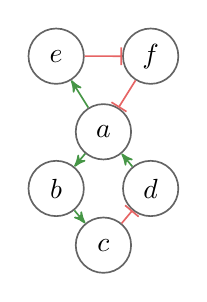
\begin{tikzpicture}[->,semithick,>=stealth',scale=1.2]
    \tikzstyle{node}=[draw=node_gray, circle, minimum size=2.0em, fill=none,text=black]

    \node[node] (a) at (0,0)       {$a$};
    \node[node] (b) at (-0.5,-0.6) {$b$};
    \node[node] (c) at (-0.0,-1.2) {$c$};
    \node[node] (d) at (0.5,-0.6)  {$d$};  
    \node[node] (e) at (-0.5,0.8)  {$e$};
    \node[node] (f) at (0.5,0.8)   {$f$};
    \path
     (a) edge[edge_green] (b)
     (b) edge[edge_green] (c)
     (c) edge[edge_red, -|] (d)
     (d) edge[edge_green] (a)
     (a) edge[edge_green] (e)
     (e) edge[edge_red, -|] (f)
     (f) edge[edge_red, -|] (a)
     ;
  \end{tikzpicture} 
  \caption{Example of an interaction graph. Green arrows indicate positive ($\plus$) influence,
    red edges negative ($\minus$) influence.
  }
  \label{fig:ig}
\end{figure}


\section*{What are signed system changes?}

Interaction graphs are an abstraction of dynamic
 quantitative systems where a quantitative state of the system is a mapping 
 $S_i : V \rightarrow \mathbb{R}^+$.
Sign consistency methods use signs to denote changes in the variables of the modeled system. 
Examples for such changes could be increased or decreased in metabolite concentrations or expression levels of genes.
The signs $\plus$ and $\minus$ are used to denote increase and decrease and 0 signifies no-change.
Sign consistency methods relate the IG model of the system and the variations in between system states
 by representing the variations as labels on the nodes in the graph. 
For example, the changes between two states of the system 
 can be represented as a sign labeling of the IG. 
Given two system states $S_R$ and $S_O$
 the differences between these states can be represented as the labeling $\mu_{RO} : V \rightarrow \{\plus, \minus, 0\}$ with
$\mu_{RO}(x) = sign(x_{S_O} - x_{S_R})$.
See Figure~\ref{fig:state_change} for an example of two states and the corresponding sign labeling.
We use the colors 
 \textcolor{edge_green}{$\blacksquare$},
 \textcolor{edge_red}{$\blacksquare$},
 \textcolor{edge_blue}{$\blacksquare$}
 to represent the signs $\plus, \minus, 0$.

\begin{figure}
  \centering
  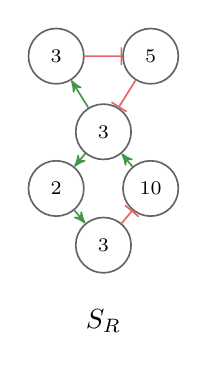
\begin{tikzpicture}[->,semithick,>=stealth',scale=1.2]
    \tikzstyle{node}=[draw=node_gray, circle, minimum size=2.0em, fill=none,text=black]

    \node[node] (a) at (0,0)       {\scriptsize $3$};
    \node[node] (b) at (-0.5,-0.6) {\scriptsize $2$};
    \node[node] (c) at (-0.0,-1.2) {\scriptsize $3$};
    \node[node] (d) at (0.5,-0.6)  {\scriptsize $10$};  
    \node[node] (e) at (-0.5,0.8)  {\scriptsize $3$};
    \node[node] (f) at (0.5,0.8)   {\scriptsize $5$};
    \node[]               (l) at (0,-2.0)    {$S_R$};

    \path
     (a) edge[edge_green] (b)
     (b) edge[edge_green] (c)
     (c) edge[edge_red, -|] (d)
     (d) edge[edge_green] (a)
     (a) edge[edge_green] (e)
     (e) edge[edge_red, -|] (f)
     (f) edge[edge_red, -|] (a)
     ;
  \end{tikzpicture} 
  ~~~~~ 
  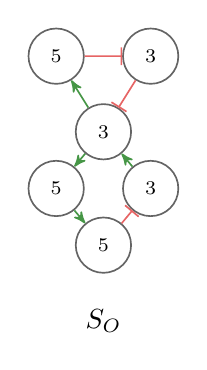
\begin{tikzpicture}[->,semithick,>=stealth',scale=1.2]
    \tikzstyle{node}=[draw=node_gray, circle, minimum size=2.0em, fill=none,text=black]

    \node[node] (a) at (0,0)       {\scriptsize $3$};
    \node[node] (b) at (-0.5,-0.6) {\scriptsize $5$};
    \node[node] (c) at (-0.0,-1.2) {\scriptsize $5$};
    \node[node] (d) at (0.5,-0.6)  {\scriptsize $3$};  
    \node[node] (e) at (-0.5,0.8)  {\scriptsize $5$};
    \node[node] (f) at (0.5,0.8)   {\scriptsize $3$};
    \node[]               (l) at (0,-2.0)    {$S_O$};

    \path
     (a) edge[edge_green] (b)
     (b) edge[edge_green] (c)
     (c) edge[edge_red, -|] (d)
     (d) edge[edge_green] (a)
     (a) edge[edge_green] (e)
     (e) edge[edge_red, -|] (f)
     (f) edge[edge_red, -|] (a)
     ;
  \end{tikzpicture}  
  ~~~~~ 
  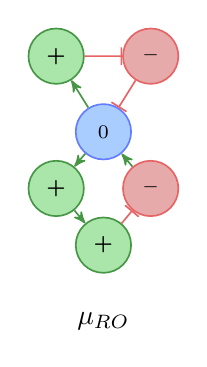
\begin{tikzpicture}[->,semithick,>=stealth',scale=1.2]
    \tikzstyle{node}=[draw=node_gray, circle, minimum size=2.0em, fill=none,text=black]
    \tikzstyle{up}=[style=node,text=black,text opacity=1,fill=node_green,draw=edge_green]
    \tikzstyle{dn}=[style=node,text=black,text opacity=1,fill=node_red,draw=edge_red]
    \tikzstyle{zn}=[style=node,text=black,text opacity=1,fill=node_blue,draw=edge_blue]

    \node[zn] (a) at (0,0)       {\scriptsize $0$};
    \node[up] (b) at (-0.5,-0.6) {\scriptsize $\plus$};
    \node[up] (c) at (-0.0,-1.2) {\scriptsize $\plus$};
    \node[dn] (d) at (0.5,-0.6)  {\scriptsize $\minus$};  
    \node[up] (e) at (-0.5,0.8)  {\scriptsize $\plus$};
    \node[dn] (f) at (0.5,0.8)   {\scriptsize $\minus$};
    \node[]               (l) at (0,-2.0)    {$\mu_{RO} $};

    \path
     (a) edge[edge_green] (b)
     (b) edge[edge_green] (c)
     (c) edge[edge_red, -|] (d)
     (d) edge[edge_green] (a)
     (a) edge[edge_green] (e)
     (e) edge[edge_red, -|] (f)
     (f) edge[edge_red, -|] (a)
     ;
  \end{tikzpicture} 
  \caption{Example of a sign labeling representing the change between two quantitative states.
  }
  \label{fig:state_change}
\end{figure}

Further, sign consistency methods define rules that determine which labelings 
of the graph are considered consistent and which are considered inconsistent.
There exist several consistency rules which are useful to model different 
properties of a biological system. 
For now, we only consider the following.

\begin{srule}[backwards propagation]
\label{rule_bw}
{\upshape Every change in a node must be explained by a change in one of its predecessors.}

Let $(V, E, \sigma)$ be an IG.
Then a labeling $\mu : V \rightarrow \{\plus, \minus, 0\}$ satisfies Rule~\ref{rule_bw} for node $i \in V$ iff
\begin{itemize}
 \item $\mu(i) = 0$, or
 \item there is some edge $j \rightarrow i$ in $E$ 
       such that $\mu(i)=\mu(j)\sigma(j,i)$.
\end{itemize}

 
\end{srule}

Rule~\ref{rule_bw} implements backward reasoning.
Given an effect we look backwards to verify its cause.
Labelings that are consistent with this rule represent the differences between steady states.
In a steady state the values of all state variables are balanced. 
Hence, the change in one variable must be sustained by the change in one of its predecessors.
In other words,
 if $S_R$ and $S_O$ are steady states of the system
 then the labeling $\mu_{RO}$ is consistent with Rule~\ref{rule_bw}.
The trivial example is when both states are the same $S_R = S_O$ then nothing changes $\forall x \in V : \mu_{RO}(x) = 0$.

Let's see what else we can do with that. 
Figure~\ref{fig:ig_labeled} shows an interaction graph and all labelings $\mu_i : V \rightarrow \{\plus, \minus, 0\}$ with $\mu_i(a)=\plus$ 
that satisfy Rule~\ref{rule_bw}.

\begin{figure}
 \begin{center}
  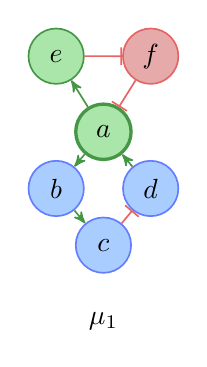
\begin{tikzpicture}[->,semithick,>=stealth',scale=1.2]
    \tikzstyle{node}=[draw=node_gray, circle, minimum size=2.0em, fill=none,text=black]
    \tikzstyle{up}=[style=node,text=black,text opacity=1,fill=node_green,draw=edge_green]
    \tikzstyle{dn}=[style=node,text=black,text opacity=1,fill=node_red,draw=edge_red]
    \tikzstyle{zn}=[style=node,text=black,text opacity=1,fill=node_blue,draw=edge_blue]

    \node[up, very thick] (a) at (0,0)       {$a$};
    \node[zn]             (b) at (-0.5,-0.6) {$b$};
    \node[zn]             (c) at (-0.0,-1.2) {$c$};
    \node[zn]             (d) at (0.5,-0.6)  {$d$};  
    \node[up]             (e) at (-0.5,0.8)  {$e$};
    \node[dn]             (f) at (0.5,0.8)   {$f$};
    \node[]               (l) at (0,-2.0)    {$\mu_1$};

    \path
     (a) edge[edge_green] (b)
     (b) edge[edge_green] (c)
     (c) edge[edge_red, -|] (d)
     (d) edge[edge_green] (a)
     (a) edge[edge_green] (e)
     (e) edge[edge_red, -|] (f)
     (f) edge[edge_red, -|] (a)
     ;
  \end{tikzpicture}
  ~~~~~
  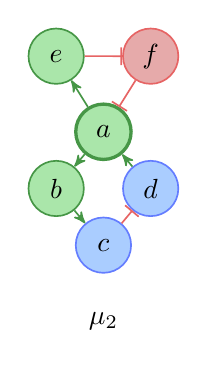
\begin{tikzpicture}[->,semithick,>=stealth',scale=1.2]
    \tikzstyle{node}=[draw=node_gray, circle, minimum size=2.0em, fill=none,text=black]
    \tikzstyle{up}=[style=node,text=black,text opacity=1,fill=node_green,draw=edge_green]
    \tikzstyle{dn}=[style=node,text=black,text opacity=1,fill=node_red,draw=edge_red]
    \tikzstyle{zn}=[style=node,text=black,text opacity=1,fill=node_blue,draw=edge_blue]

    \node[up, very thick] (a) at (0,0)       {$a$};
    \node[up] (b) at (-0.5,-0.6) {$b$};
    \node[zn] (c) at (-0.0,-1.2) {$c$};
    \node[zn] (d) at (0.5,-0.6)  {$d$};  
    \node[up] (e) at (-0.5,0.8)  {$e$};
    \node[dn] (f) at (0.5,0.8)   {$f$};
    \node[]               (l) at (0,-2.0)    {$\mu_2$};

    \path
     (a) edge[edge_green] (b)
     (b) edge[edge_green] (c)
     (c) edge[edge_red, -|] (d)
     (d) edge[edge_green] (a)
     (a) edge[edge_green] (e)
     (e) edge[edge_red, -|] (f)
     (f) edge[edge_red, -|] (a)
     ;
  \end{tikzpicture}
  ~~~~~  
  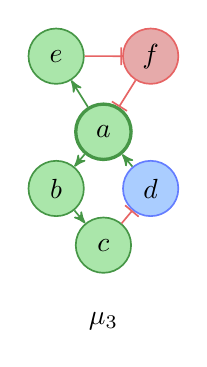
\begin{tikzpicture}[->,semithick,>=stealth',scale=1.2]
    \tikzstyle{node}=[draw=node_gray, circle, minimum size=2.0em, fill=none,text=black]
    \tikzstyle{up}=[style=node,text=black,text opacity=1,fill=node_green,draw=edge_green]
    \tikzstyle{dn}=[style=node,text=black,text opacity=1,fill=node_red,draw=edge_red]
    \tikzstyle{zn}=[style=node,text=black,text opacity=1,fill=node_blue,draw=edge_blue]

    \node[up, very thick] (a) at (0,0)       {$a$};
    \node[up] (b) at (-0.5,-0.6) {$b$};
    \node[up] (c) at (-0.0,-1.2) {$c$};
    \node[zn] (d) at (0.5,-0.6)  {$d$};  
    \node[up] (e) at (-0.5,0.8)  {$e$};
    \node[dn] (f) at (0.5,0.8)   {$f$};
    \node[]               (l) at (0,-2.0)    {$\mu_3$};
    
    \path
     (a) edge[edge_green] (b)
     (b) edge[edge_green] (c)
     (c) edge[edge_red, -|] (d)
     (d) edge[edge_green] (a)
     (a) edge[edge_green] (e)
     (e) edge[edge_red, -|] (f)
     (f) edge[edge_red, -|] (a)
     ;
  \end{tikzpicture}
  ~~~~~  
  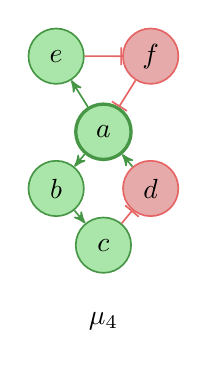
\begin{tikzpicture}[->,semithick,>=stealth',scale=1.2]
    \tikzstyle{node}=[draw=node_gray, circle, minimum size=2.0em, fill=none,text=black]
    \tikzstyle{up}=[style=node,text=black,text opacity=1,fill=node_green,draw=edge_green]
    \tikzstyle{dn}=[style=node,text=black,text opacity=1,fill=node_red,draw=edge_red]
    \tikzstyle{zn}=[style=node,text=black,text opacity=1,fill=node_blue,draw=edge_blue]

    \node[up, very thick] (a) at (0,0)       {$a$};
    \node[up] (b) at (-0.5,-0.6) {$b$};
    \node[up] (c) at (-0.0,-1.2) {$c$};
    \node[dn] (d) at (0.5,-0.6)  {$d$};  
    \node[up] (e) at (-0.5,0.8)  {$e$};
    \node[dn] (f) at (0.5,0.8)   {$f$};
    \node[]               (l) at (0,-2.0)    {$\mu_4$};

    \path
     (a) edge[edge_green] (b)
     (b) edge[edge_green] (c)
     (c) edge[edge_red, -|] (d)
     (d) edge[edge_green] (a)
     (a) edge[edge_green] (e)
     (e) edge[edge_red, -|] (f)
     (f) edge[edge_red, -|] (a)
     ;
  \end{tikzpicture}   
\end{center}
\caption{Labeled interaction graph}
\label{fig:ig_labeled}
\end{figure}


Often it is useful to represent the labelings in a table as shown in Table~\ref{tab:labeled}.
As you can see, there exist only four labelings that satisfy these constraints. 
In every of these labeling it holds $\mu_i(e)=\plus$ and $\mu_i(f)=\minus$.
We can use this table to predict the behavior of the system.
We see that in every steady state, with an increase in $a$ we also have an increase in $e$ and a decrease in $f$.
For $b$ and $c$ we can predict that they will not decrease,
 and for $d$ that it will not increase.

\begin{table}
\centering
\definecolor{dark}{RGB}{115,115,115} 
\newcommand\gr{\cellcolor{node_green}{\scriptsize $\plus$}}
\newcommand\ro{\cellcolor{node_red}{\scriptsize $\minus$}}
\newcommand\bl{\cellcolor{node_blue}{\scriptsize $0$}}

\setlength\tabcolsep{2.2pt}
\begin{tabular}{l ccccc|}
%  & \multicolumn{5}{c}{admissible labelings} \\
\multicolumn{1}{l|}{}   & $\mu_1$&$\mu_2$&$\mu_3$&$\mu_4$  \\
\hline
\multicolumn{1}{l|}{$a$}   & \gr&\gr&\gr&\gr  \\
% \hline
\multicolumn{1}{l|}{$b$}   & \bl&\gr&\gr&\gr  \\
\multicolumn{1}{l|}{$c$}   & \bl&\bl&\gr&\gr  \\
\multicolumn{1}{l|}{$d$~~} & \bl&\bl&\bl&\ro  \\
\multicolumn{1}{l|}{$e$~~} & \gr&\gr&\gr&\gr  \\
\multicolumn{1}{l|}{$f$~~} & \ro&\ro&\ro&\ro  \\
% \hline
\end{tabular} 
\bigskip
\caption{Table of admissible labelings.}
\label{tab:labeled} 
\end{table}


\section*{Conclusion}

In this part I introduced interaction graphs and explained how they can be used to model biological systems.
We have seen how sign consistency methods represent variations in the system as sign labelings,
and how sign consistency constraints can be used to derive predictions over the steady states of a system.
So far we have modeled a closed system.
In Part~2 I will introduce external inputs and perturbations.



% \bibliographystyle{abbrv}
% \bibliography{local} 

\chapter*{Predicting system responses to perturbations}
\addcontentsline{toc}{chapter}{Predicting system responses to perturbations}
In Part~1 of this series we learned how to use interaction graphs and sign consistency methods
 to reason about steady states in closed systems.
In this part we add external influences to our model and answer the question
 how a biological system responds to external influences.


\section*{Inputs and perturbations}

Most systems interact in some ways with a surrounding context i.e. their environment.
The interface to the environment is provided by variables which are not controlled by the modeled system itself but externally.
We call variables in our system which are controlled externally \emph{inputs} and
 we denote the set of nodes that represent input variables with $I \subseteq V$.
Because input nodes are controlled externally, they are excluded from the sign consistency rules.

For the closed system shown in Figure~\ref{fig:ig},
 there exists no single labeling $\mu: V \rightarrow \{\plus, \minus, 0\}$,
 with $\mu(a)=\plus$ and $\mu(b)=\minus$ that satisfies Rule~\ref{rule_bw} for all $v \in V$.
%
In other words, there exists no transition between steady states where $a$ increases and $b$ decreases.
Because $a$ is the only predecessor of $b$, between all steady states changes in $a$ and $b$ must have the same sign.

\begin{figure}
  \centering
  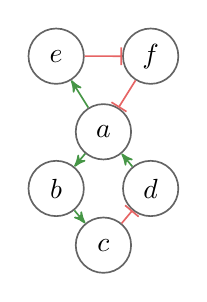
\begin{tikzpicture}[->,semithick,>=stealth',scale=1.2]
    \tikzstyle{node}=[draw=node_gray, circle, minimum size=2.0em, fill=none,text=black]

    \node[node] (a) at (0,0)       {$a$};
    \node[node] (b) at (-0.5,-0.6) {$b$};
    \node[node] (c) at (-0.0,-1.2) {$c$};
    \node[node] (d) at (0.5,-0.6)  {$d$};  
    \node[node] (e) at (-0.5,0.8)  {$e$};
    \node[node] (f) at (0.5,0.8)   {$f$};

    \path
     (a) edge[edge_green] (b)
     (b) edge[edge_green] (c)
     (c) edge[edge_red, -|] (d)
     (d) edge[edge_green] (a)
     (a) edge[edge_green] (e)
     (e) edge[edge_red, -|] (f)
     (f) edge[edge_red, -|] (a)
     ;
  \end{tikzpicture}
  \caption{Example of an interaction graph. Green arrows indicate positive ($\plus$) influence,
    red edges negative ($\minus$) influence.
  } 
  \label{fig:ig}
\end{figure}

We can interpret our model as an open system,
 were the value of $b$ is determined by the environment by declaring $b$ as a input variable.
With perturbations we can now take control over the input variables and find out how the system behaves under different environmental conditions.
For example we can now find out how our system reacts to a decrease in $b$.
Figure~\ref{fig:ig_labeled2} shows all labelings $\mu_i$ that satisfy Rule~\ref{rule_bw} for all $v\in V \setminus I$ with 
$I=\{b\}$ and $\mu_i(a)=\plus$ and $\mu_i(b)=\minus$. 
Input nodes are denoted with a black incoming arrow.

\begin{figure}
 \begin{center}
  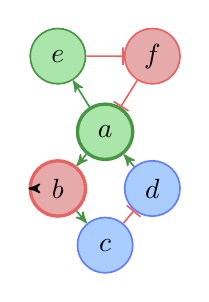
\begin{tikzpicture}[->,semithick,>=stealth',scale=1.2]
    \tikzstyle{node}=[draw=node_gray, circle, minimum size=2.0em, fill=none,text=black]
    \tikzstyle{up}=[style=node,text=black,text opacity=1,fill=node_green,draw=edge_green]
    \tikzstyle{dn}=[style=node,text=black,text opacity=1,fill=node_red,draw=edge_red]
    \tikzstyle{zn}=[style=node,text=black,text opacity=1,fill=node_blue,draw=edge_blue]

    \node[up, very thick] (a) at (0,0)       {$a$};
    \node[dn, very thick] (b) at (-0.5,-0.6) {$b$};
    \node[zn]             (c) at (-0.0,-1.2) {$c$};
    \node[zn]             (d) at (0.5,-0.6)  {$d$};  
    \node[up]             (e) at (-0.5,0.8)  {$e$};
    \node[dn]             (f) at (0.5,0.8)   {$f$};
%     \node[]               (l) at (0,-2.0)    {$\mu_1$};

    \path
     (-0.8,-0.6) edge (b)
     (a) edge[edge_green] (b)
     (b) edge[edge_green] (c)
     (c) edge[edge_red, -|] (d)
     (d) edge[edge_green] (a)
     (a) edge[edge_green] (e)
     (e) edge[edge_red, -|] (f)
     (f) edge[edge_red, -|] (a)
     ;
  \end{tikzpicture}
  ~~~~
  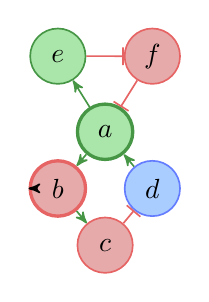
\begin{tikzpicture}[->,semithick,>=stealth',scale=1.2]
    \tikzstyle{node}=[draw=node_gray, circle, minimum size=2.0em, fill=none,text=black]
    \tikzstyle{up}=[style=node,text=black,text opacity=1,fill=node_green,draw=edge_green]
    \tikzstyle{dn}=[style=node,text=black,text opacity=1,fill=node_red,draw=edge_red]
    \tikzstyle{zn}=[style=node,text=black,text opacity=1,fill=node_blue,draw=edge_blue]

    \node[up, very thick] (a) at (0,0)       {$a$};
    \node[dn, very thick] (b) at (-0.5,-0.6) {$b$};
    \node[dn] (c) at (-0.0,-1.2) {$c$};
    \node[zn] (d) at (0.5,-0.6)  {$d$};  
    \node[up] (e) at (-0.5,0.8)  {$e$};
    \node[dn] (f) at (0.5,0.8)   {$f$};
%     \node[]               (l) at (0,-2.0)    {$\mu_2$};

    \path
     (-0.8,-0.6) edge (b)
     (a) edge[edge_green] (b)
     (b) edge[edge_green] (c)
     (c) edge[edge_red, -|] (d)
     (d) edge[edge_green] (a)
     (a) edge[edge_green] (e)
     (e) edge[edge_red, -|] (f)
     (f) edge[edge_red, -|] (a)
     ;
  \end{tikzpicture}
  ~~~~  
  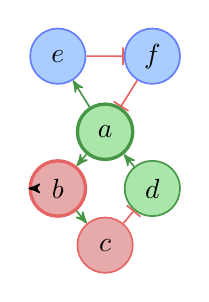
\begin{tikzpicture}[->,semithick,>=stealth',scale=1.2]
    \tikzstyle{node}=[draw=node_gray, circle, minimum size=2.0em, fill=none,text=black]
    \tikzstyle{up}=[style=node,text=black,text opacity=1,fill=node_green,draw=edge_green]
    \tikzstyle{dn}=[style=node,text=black,text opacity=1,fill=node_red,draw=edge_red]
    \tikzstyle{zn}=[style=node,text=black,text opacity=1,fill=node_blue,draw=edge_blue]

    \node[up, very thick] (a) at (0,0)       {$a$};
    \node[dn, very thick] (b) at (-0.5,-0.6) {$b$};
    \node[dn] (c) at (-0.0,-1.2) {$c$};
    \node[up] (d) at (0.5,-0.6)  {$d$};  
    \node[zn] (e) at (-0.5,0.8)  {$e$};
    \node[zn] (f) at (0.5,0.8)   {$f$};
%     \node[]               (l) at (0,-2.0)    {$\mu_3$};

    \path
     (-0.8,-0.6) edge (b)
     (a) edge[edge_green] (b)
     (b) edge[edge_green] (c)
     (c) edge[edge_red, -|] (d)
     (d) edge[edge_green] (a)
     (a) edge[edge_green] (e)
     (e) edge[edge_red, -|] (f)
     (f) edge[edge_red, -|] (a)
     ;
  \end{tikzpicture}  
  ~~~~  
  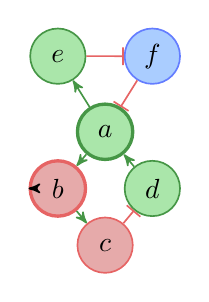
\begin{tikzpicture}[->,semithick,>=stealth',scale=1.2]
    \tikzstyle{node}=[draw=node_gray, circle, minimum size=2.0em, fill=none,text=black]
    \tikzstyle{up}=[style=node,text=black,text opacity=1,fill=node_green,draw=edge_green]
    \tikzstyle{dn}=[style=node,text=black,text opacity=1,fill=node_red,draw=edge_red]
    \tikzstyle{zn}=[style=node,text=black,text opacity=1,fill=node_blue,draw=edge_blue]

    \node[up, very thick] (a) at (0,0)       {$a$};
    \node[dn, very thick] (b) at (-0.5,-0.6) {$b$};
    \node[dn] (c) at (-0.0,-1.2) {$c$};
    \node[up] (d) at (0.5,-0.6)  {$d$};  
    \node[up] (e) at (-0.5,0.8)  {$e$};
    \node[zn] (f) at (0.5,0.8)   {$f$};
%     \node[]               (l) at (0,-2.0)    {$\mu_4$};

    \path
     (-0.8,-0.6) edge (b)
     (a) edge[edge_green] (b)
     (b) edge[edge_green] (c)
     (c) edge[edge_red, -|] (d)
     (d) edge[edge_green] (a)
     (a) edge[edge_green] (e)
     (e) edge[edge_red, -|] (f)
     (f) edge[edge_red, -|] (a)
     ;
  \end{tikzpicture}
  ~~~~
  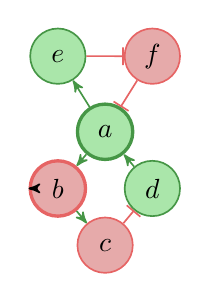
\begin{tikzpicture}[->,semithick,>=stealth',scale=1.2]
    \tikzstyle{node}=[draw=node_gray, circle, minimum size=2.0em, fill=none,text=black]
    \tikzstyle{up}=[style=node,text=black,text opacity=1,fill=node_green,draw=edge_green]
    \tikzstyle{dn}=[style=node,text=black,text opacity=1,fill=node_red,draw=edge_red]
    \tikzstyle{zn}=[style=node,text=black,text opacity=1,fill=node_blue,draw=edge_blue]

    \node[up, very thick] (a) at (0,0)       {$a$};
    \node[dn, very thick] (b) at (-0.5,-0.6) {$b$};
    \node[dn] (c) at (-0.0,-1.2) {$c$};
    \node[up] (d) at (0.5,-0.6)  {$d$};  
    \node[up] (e) at (-0.5,0.8)  {$e$};
    \node[dn] (f) at (0.5,0.8)   {$f$};
%     \node[]               (l) at (0,-2.0)    {$\mu_5$};
    
    \path
     (-0.8,-0.6) edge (b)
     (a) edge[edge_green] (b)
     (b) edge[edge_green] (c)
     (c) edge[edge_red, -|] (d)
     (d) edge[edge_green] (a)
     (a) edge[edge_green] (e)
     (e) edge[edge_red, -|] (f)
     (f) edge[edge_red, -|] (a)
     ;
  \end{tikzpicture}   
\end{center}
\caption{Labeled interaction graph}
\label{fig:ig_labeled2}
\end{figure}


We see that using a perfect perturbation, a sustained decrease of $b$,
 the system can reach a quasi steady state where both $a$ and $d$ are increased.
This is a state which could not be reached in the closed system without perturbation.
While this is already an interesting reasoning mode,
 it is even more interesting to flip the question around and use this approach to do some treatment planning.
Let's see, what are the minimal perturbations that would allow the system to transition 
 into a state where $a$ and $d$ are increased?
Figure~\ref{fig:ig_labeled3} shows the potential perturbations (along with partial labelings) that allow for such a state-transition.
We can see that we have two more alternatives to reach our goal, either a direct increase in $d$ or a decrease in $c$.
 
\begin{figure}
 \begin{center}
  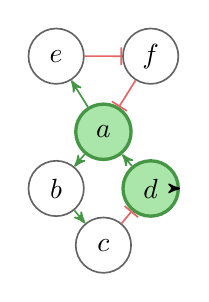
\begin{tikzpicture}[->,semithick,>=stealth',scale=1.2]
    \tikzstyle{node}=[draw=node_gray, circle, minimum size=2.0em, fill=none,text=black]
    \tikzstyle{up}=[style=node,text=black,text opacity=1,fill=node_green,draw=edge_green]
    \tikzstyle{dn}=[style=node,text=black,text opacity=1,fill=node_red,draw=edge_red]
    \tikzstyle{zn}=[style=node,text=black,text opacity=1,fill=node_blue,draw=edge_blue]

    \node[up, very thick] (a) at (0,0)       {$a$};
    \node[node]             (b) at (-0.5,-0.6) {$b$};
    \node[node]             (c) at (-0.0,-1.2) {$c$};
    \node[up, very thick] (d) at (0.5,-0.6)  {$d$};  
    \node[node]             (e) at (-0.5,0.8)  {$e$};
    \node[node]             (f) at (0.5,0.8)   {$f$};
%     \node[]               (l) at (0,-2.0)    {$\mu_1$};

    \path
     (0.8,-0.6) edge (d)
     (a) edge[edge_green] (b)
     (b) edge[edge_green] (c)
     (c) edge[edge_red, -|] (d)
     (d) edge[edge_green] (a)
     (a) edge[edge_green] (e)
     (e) edge[edge_red, -|] (f)
     (f) edge[edge_red, -|] (a)
     ;
  \end{tikzpicture}
  ~~~~
  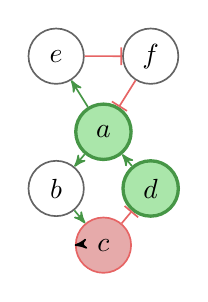
\begin{tikzpicture}[->,semithick,>=stealth',scale=1.2]
    \tikzstyle{node}=[draw=node_gray, circle, minimum size=2.0em, fill=none,text=black]
    \tikzstyle{up}=[style=node,text=black,text opacity=1,fill=node_green,draw=edge_green]
    \tikzstyle{dn}=[style=node,text=black,text opacity=1,fill=node_red,draw=edge_red]
    \tikzstyle{zn}=[style=node,text=black,text opacity=1,fill=node_blue,draw=edge_blue]

    \node[up, very thick] (a) at (0,0)       {$a$};
    \node[node]               (b) at (-0.5,-0.6) {$b$};
    \node[dn]             (c) at (-0.0,-1.2) {$c$};
    \node[up, very thick] (d) at (0.5,-0.6)  {$d$};  
    \node[node]               (e) at (-0.5,0.8)  {$e$};
    \node[node]               (f) at (0.5,0.8)   {$f$};
%     \node[]               (l) at (0,-2.0)    {$\mu_2$};

    \path
     (-0.3,-1.2) edge (c)
     (a) edge[edge_green] (b)
     (b) edge[edge_green] (c)
     (c) edge[edge_red, -|] (d)
     (d) edge[edge_green] (a)
     (a) edge[edge_green] (e)
     (e) edge[edge_red, -|] (f)
     (f) edge[edge_red, -|] (a)
     ;
  \end{tikzpicture}
  ~~~~
  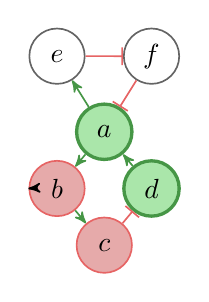
\begin{tikzpicture}[->,semithick,>=stealth',scale=1.2]
    \tikzstyle{node}=[draw=node_gray, circle, minimum size=2.0em, fill=none,text=black]
    \tikzstyle{up}=[style=node,text=black,text opacity=1,fill=node_green,draw=edge_green]
    \tikzstyle{dn}=[style=node,text=black,text opacity=1,fill=node_red,draw=edge_red]
    \tikzstyle{zn}=[style=node,text=black,text opacity=1,fill=node_blue,draw=edge_blue]

    \node[up, very thick] (a) at (0,0)       {$a$};
    \node[dn]             (b) at (-0.5,-0.6) {$b$};
    \node[dn]             (c) at (-0.0,-1.2) {$c$};
    \node[up, very thick] (d) at (0.5,-0.6)  {$d$};  
    \node[node]               (e) at (-0.5,0.8)  {$e$};
    \node[node]               (f) at (0.5,0.8)   {$f$};
%     \node[]               (l) at (0,-2.0)    {$\mu_3$};

    \path
     (-0.8,-0.6) edge (b)
     (a) edge[edge_green] (b)
     (b) edge[edge_green] (c)
     (c) edge[edge_red, -|] (d)
     (d) edge[edge_green] (a)
     (a) edge[edge_green] (e)
     (e) edge[edge_red, -|] (f)
     (f) edge[edge_red, -|] (a)
     ;
  \end{tikzpicture}
  
\end{center}
\caption{Minimal perturbations of the system that can results in an increase of $a$ and $d$ (along with partial labeling)}
\label{fig:ig_labeled3}
\end{figure}

\section*{Perturbations and model topology}

Perturbations play a major role in the analysis of biological models.
A complementary view point on perturbations is that they allow us to alter the model structure.
In particular, all incoming edges of an input node can be ignored because the node is no longer constrained by the system but by us.
A special role play so called 0-perturbations, 
 these are perturbations were the value of a variable is kept constant over the state transition.
For those nodes the only possible label is 0 and we can ignore their outgoing edges because they can't be responsible for any downstream changes.
It's easy to see that for complex models with many cyclic interactions such perturbations are very useful
 to investigate the influence of single components while excluding the influence of others.
In a later part, we will see how perturbations are used to design experiments that allow to discriminate among alternative model topologies.

\section*{Conclusion}

In this part I introduced inputs and we have seen how one can model perturbations of a system.
We have seen how we can reason over possible perturbations of a systems, and how to use this for treatment planning.
In the next part I will introduce a new consistency rule that allows us to handle constraints that are posed by minima or maxima of system variables.


\chapter*{Minimum and Maximum level constraints}
\addcontentsline{toc}{chapter}{Minimum and Maximum level constraints}
Previously, we covered the sign consistency rule for backward propagation.
In this part I will introduce a new rule that discards solutions that
violate minimum and maximum constraints on system variables.

 
\section*{Constrained values for system variables} 

A lot of variables in biological systems have minimum (resp. maximum) constraints.
Concentration level cannot go below $0$ or above $100\%$, and 
signals which are below the detection threshold cannot drop any further.
Figure~\ref{fig:minmax} shows an IG with $4$ variables $a$, $b$, $c$ and $d$. 
Let's say the variable $c$ represent a concentration and only values in the range of $0$ to $100$ are valid.
Further, we know that in our reference state $S_R$ the variable $c$ is at its minimum.
Let's try to find all labelings $\mu_{i}$ that represent transitions from $S_R$ to a state $S_i$ 
 where the level of $d$ has increased, $\mu_{i}(d)=\plus$.
Figure~\ref{fig:minmaxlabelings} shows all labelings $\mu_{i}$ that satisfy consistency Rule~\ref{rule_bw}.
The labelings $\mu_2$ and $\mu_3$ violate the minimum constraint on variable $c$, 
 because there exists no value for $c$ in $[0,100]$ such that $ sign(c-0)=\minus$.


\begin{figure}\label{fig:minmax}
\centering
  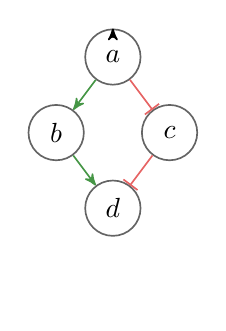
\begin{tikzpicture}[->,semithick,>=stealth',scale=1.2]
    \tikzstyle{node}=[draw=node_gray, circle, minimum size=2.0em, fill=none,text=black]
    \tikzstyle{up}=[style=node,text=black,text opacity=1,fill=node_green,draw=edge_green]
    \tikzstyle{dn}=[style=node,text=black,text opacity=1,fill=node_red,draw=edge_red]
    \tikzstyle{zn}=[style=node,text=black,text opacity=1,fill=node_blue,draw=edge_blue]

    \node[node] (a) at (0,0)       {$a$};
    \node[node] (b) at (-0.6,-0.8) {$b$};
    \node[node] (c) at ( 0.6,-0.8) {$c$};
    \node[node] (d) at (0,-1.6)    {$d$};
    \node[text=white]     (l) at (0,-2.4)    {O};
    \path
     (0,0.3) edge (a)
     (a) edge[edge_green]  (b)
     (a) edge[edge_red,-|] (c)     
     (b) edge[edge_green]  (d)
     (c) edge[edge_red,-|] (d)   
     ;
  \end{tikzpicture}
  ~~~~~  
  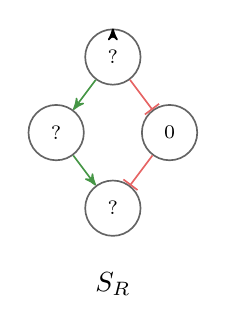
\begin{tikzpicture}[->,semithick,>=stealth',scale=1.2]
    \tikzstyle{node}=[draw=node_gray, circle, minimum size=2.0em, fill=none,text=black]
    \tikzstyle{up}=[style=node,text=black,text opacity=1,fill=node_green,draw=edge_green]
    \tikzstyle{dn}=[style=node,text=black,text opacity=1,fill=node_red,draw=edge_red]
    \tikzstyle{zn}=[style=node,text=black,text opacity=1,fill=node_blue,draw=edge_blue]

    \node[node] (a) at (0,0)       {\scriptsize ?};
    \node[node] (b) at (-0.6,-0.8) {\scriptsize ?};
    \node[node] (c) at ( 0.6,-0.8) {\scriptsize $0$};
    \node[node] (d) at (0,-1.6)    {\scriptsize ?};
    \node[]     (l) at (0,-2.4)    {$S_R $};
    \path
     (0,0.3) edge (a)
     (a) edge[edge_green]  (b)
     (a) edge[edge_red,-|] (c)     
     (b) edge[edge_green]  (d)
     (c) edge[edge_red,-|] (d)   
     ;
  \end{tikzpicture}
  \caption{An IG and with the reference state $S_R$ where variable $c$ on its minimum.}
\end{figure}  

\begin{figure}\label{fig:minmaxlabelings}
\centering
  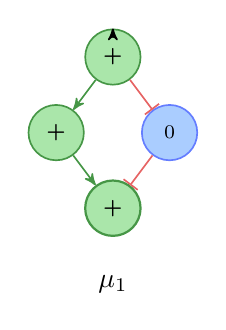
\begin{tikzpicture}[->,semithick,>=stealth',scale=1.2]
    \tikzstyle{node}=[draw=node_gray, circle, minimum size=2.0em, fill=none,text=black]
    \tikzstyle{up}=[style=node,text=black,text opacity=1,fill=node_green,draw=edge_green]
    \tikzstyle{dn}=[style=node,text=black,text opacity=1,fill=node_red,draw=edge_red]
    \tikzstyle{zn}=[style=node,text=black,text opacity=1,fill=node_blue,draw=edge_blue]

    \node[up] (a) at (0,0)       {\scriptsize $\plus$};
    \node[up] (b) at (-0.6,-0.8) {\scriptsize $\plus$};
    \node[zn] (c) at ( 0.6,-0.8) {\scriptsize $0$};
    \node[thick,up] (d) at (0,-1.6)    {\scriptsize $\plus$};
    \node[]   (l) at (0,-2.4)    {$\mu_1$};
    \path
     (0,0.3) edge (a)
     (a) edge[edge_green]  (b)
     (a) edge[edge_red,-|] (c)     
     (b) edge[edge_green]  (d)
     (c) edge[edge_red,-|] (d)   
     ;
  \end{tikzpicture}
  ~~~~~  
  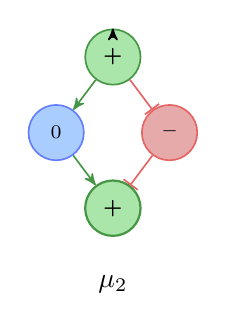
\begin{tikzpicture}[->,semithick,>=stealth',scale=1.2]
    \tikzstyle{node}=[draw=node_gray, circle, minimum size=2.0em, fill=none,text=black]
    \tikzstyle{up}=[style=node,text=black,text opacity=1,fill=node_green,draw=edge_green]
    \tikzstyle{dn}=[style=node,text=black,text opacity=1,fill=node_red,draw=edge_red]
    \tikzstyle{zn}=[style=node,text=black,text opacity=1,fill=node_blue,draw=edge_blue]

    \node[up] (a) at (0,0)       {\scriptsize $\plus$};
    \node[zn] (b) at (-0.6,-0.8) {\scriptsize $0$};
    \node[dn] (c) at ( 0.6,-0.8) {\scriptsize $\minus$};
    \node[thick,up] (d) at (0,-1.6)    {\scriptsize $\plus$};
    \node[]   (l) at (0,-2.4)    {$\mu_2$};
    \path
     (0,0.3) edge (a)
     (a) edge[edge_green]  (b)
     (a) edge[edge_red,-|] (c)     
     (b) edge[edge_green]  (d)
     (c) edge[edge_red,-|] (d)   
     ;
  \end{tikzpicture}
  ~~~~~  
  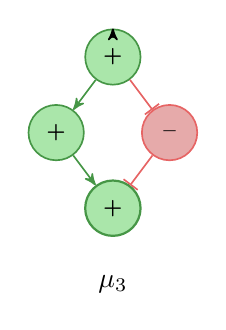
\begin{tikzpicture}[->,semithick,>=stealth',scale=1.2]
    \tikzstyle{node}=[draw=node_gray, circle, minimum size=2.0em, fill=none,text=black]
    \tikzstyle{up}=[style=node,text=black,text opacity=1,fill=node_green,draw=edge_green]
    \tikzstyle{dn}=[style=node,text=black,text opacity=1,fill=node_red,draw=edge_red]
    \tikzstyle{zn}=[style=node,text=black,text opacity=1,fill=node_blue,draw=edge_blue]

    \node[up] (a) at (0,0)       {\scriptsize $\plus$};
    \node[up] (b) at (-0.6,-0.8) {\scriptsize $\plus$};
    \node[dn] (c) at ( 0.6,-0.8) {\scriptsize $\minus$};
    \node[thick,up] (d) at (0,-1.6)    {\scriptsize $\plus$};
    \node[]   (l) at (0,-2.4)    {$\mu_3$};
    \path
     (0,0.3) edge (a)
     (a) edge[edge_green]  (b)
     (a) edge[edge_red,-|] (c)     
     (b) edge[edge_green]  (d)
     (c) edge[edge_red,-|] (d)   
     ;
  \end{tikzpicture}
  \caption{All labelings $\mu_i$ with $\mu_i(d)=\plus$ that satisfy Rule~\ref{rule_bw}. 
   Only $\mu_1$ is consistent with the value restrictions of variable $c$.}
\end{figure}

To deal with minimum (resp. maximum) constraints we introduce a new consistency rule.

\begin{srule}[obey minima/maxima]
\label{rule_minmax}
{\upshape A variable that is on its minimum cannot decrease and a variable at its maximum cannot increase.}

Let $(V, E, \sigma)$ be an IG, 
$MIN \subseteq V$ variables that are at their minimum, and  
$MAX \subseteq V$ variables that are at their maximum.
Then a labeling $\mu : V \rightarrow \{\plus, \minus, 0\}$ satisfies Rule~\ref{rule_minmax} for node $i \in V$ iff
\begin{itemize}
 \item $\mu(i) = 0$, or
 \item $\mu(i) = \minus$, and $i \notin MIN$ or 
 \item $\mu(i) = \plus$, and $i \notin MAX$.
\end{itemize}
\end{srule}

Rule~\ref{rule_minmax} allows us to exclude solutions that violate the constraints on minimal/maximal values.
In Figure~\ref{fig:minmaxlabelings} only labeling $\mu_1$ satisfies both consistency rules~\ref{rule_bw} and~\ref{rule_minmax}.

\section*{Conclusion}
In this part I introduced an consistency rule that allows us to filter solutions that violate constraints 
 restricting the minimum or maximum level of system variables.
I have shown how it can be combined with other consistency rules to get better explanations for state transitions.
In the next part I will introduce a new consistency rule that increases the predictive power of sign consistency methods.

\chapter*{Predicting effects on downstream regulated variables}
\addcontentsline{toc}{chapter}{Predicting effects on downstream regulated variables}
Previously, we covered the sign consistency rule for backward propagation
 which works for transitions between steady states.
In this part I introduce another consistency rule that also works for steady state transitions,
 and increases the predictive power of sign consistency methods.

\section*{Forward propagation}

The backward reasoning implemented by Rule~\ref{rule_bw} is very cautious. 
It expresses the assumption is that for every effect there must be a cause
 but it excludes the assumption that a change must have and effect.
Figure~\ref{fig:weak_prop} shows all labelings $\mu_i$ that are consistent with Rule~\ref{rule_bw} and were $\mu_i(b)=\plus$.
In all labelings it holds that $\mu_i(a)=\plus$, so we can predict very precisely the cause for an increase in $b$.
But the labelings for $c$ are ambiguous, although we see an increase in $b$ we cannot predict an increase in $c$.

\begin{figure}
\centering
  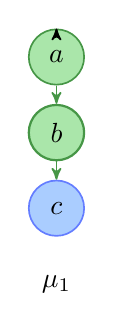
\begin{tikzpicture}[->,semithick,>=stealth',scale=1.2]
    \tikzstyle{node}=[draw=node_gray, circle, minimum size=2.0em, fill=none,text=black]
    \tikzstyle{up}=[style=node,text=black,text opacity=1,fill=node_green,draw=edge_green]
    \tikzstyle{dn}=[style=node,text=black,text opacity=1,fill=node_red,draw=edge_red]
    \tikzstyle{zn}=[style=node,text=black,text opacity=1,fill=node_blue,draw=edge_blue]

    \node[up]       (a) at (0,0)    {$a$};
    \node[up,thick] (b) at (0,-0.8) {$b$};
    \node[zn]       (c) at (0,-1.6) {$c$};
    \node[]         (l) at (0,-2.4) {$\mu_1 $};
    \path
     (0,0.3) edge (a)
     (a) edge[edge_green] (b)
     (b) edge[edge_green] (c)
     ;
  \end{tikzpicture}  
  ~~~~~  
  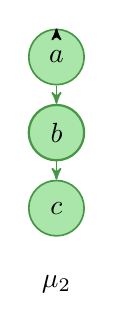
\begin{tikzpicture}[->,semithick,>=stealth',scale=1.2]
    \tikzstyle{node}=[draw=node_gray, circle, minimum size=2.0em, fill=none,text=black]
    \tikzstyle{up}=[style=node,text=black,text opacity=1,fill=node_green,draw=edge_green]
    \tikzstyle{dn}=[style=node,text=black,text opacity=1,fill=node_red,draw=edge_red]
    \tikzstyle{zn}=[style=node,text=black,text opacity=1,fill=node_blue,draw=edge_blue]

    \node[up]       (a) at (0,0)    {$a$};
    \node[up,thick] (b) at (0,-0.8) {$b$};
    \node[up]       (c) at (0,-1.6) {$c$};
    \node[]         (l) at (0,-2.4) {$\mu_2 $};
    \path
     (0,0.3) edge (a)
     (a) edge[edge_green] (b)
     (b) edge[edge_green] (c)
     ;
  \end{tikzpicture} 

\caption{Prediction under consistency Rule~1. 
  Backward propagation does not allow an unambiguous prediction for $c$.}
\label{fig:weak_prop} 
\end{figure}

To increase the predictive power of our method we define a new consistency rule 
 that implements the assumption that a change in one variable has an effect on its successors.
We define this rule for independent regulations $i \rightarrow j$ were a change in $i$ is sufficient to cause a change in $j$.
In the next part we will introduce cooperative (dependent) regulations  
 were it depends on other variables in the system whether the change in $i$ will have an effect on $j$.
 
\begin{figure}
\begin{tabular}{p{65pt}p{65pt}p{65pt}p{65pt}p{65pt}}
 \centering $S_1$ & \centering $S_2$ & \centering $S_3$ & \centering $S_4$ & \centering $S_5$ %& $S_6$
 \cr &
 \\
  \centering
  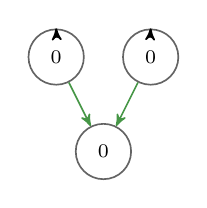
\begin{tikzpicture}[->,semithick,>=stealth',scale=1.2]
    \tikzstyle{node}=[draw=node_gray, circle, minimum size=2.0em, fill=none,text=black]
    \tikzstyle{cone}=[draw=black, circle, minimum size=1.0em, fill=none,text=black]

    \node[node] (a)  at (-0.5,0.8)  {\scriptsize $0$};
    \node[node] (b)  at (0.5,0.8)   {\scriptsize $0$};
    \node[node] (c)  at (0,-0.2)    {\scriptsize $0$};
    \path
     (-0.5,1.1) edge[] (a)
     ( 0.5,1.1) edge[] (b)
     (a) edge[edge_green] (c)
     (b) edge[edge_green] (c)
     ;
  \end{tikzpicture}
 &
  \centering
  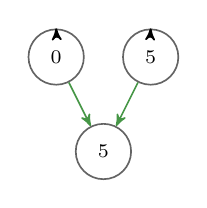
\begin{tikzpicture}[->,semithick,>=stealth',scale=1.2]
    \tikzstyle{node}=[draw=node_gray, circle, minimum size=2.0em, fill=none,text=black]
    \tikzstyle{cone}=[draw=black, circle, minimum size=1.0em, fill=none,text=black]

    \node[node] (a)  at (-0.5,0.8)  {\scriptsize $0$};
    \node[node] (b)  at (0.5,0.8)   {\scriptsize $5$};
    \node[node] (c)  at (0,-0.2)    {\scriptsize $5$};
    \path
     (-0.5,1.1) edge[] (a)
     ( 0.5,1.1) edge[] (b)
     (a) edge[edge_green] (c)
     (b) edge[edge_green] (c)
     ;
  \end{tikzpicture}
 &
  \centering
  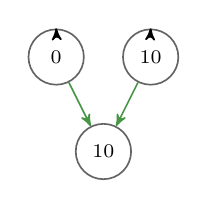
\begin{tikzpicture}[->,semithick,>=stealth',scale=1.2]
    \tikzstyle{node}=[draw=node_gray, circle, minimum size=2.0em, fill=none,text=black]
    \tikzstyle{cone}=[draw=black, circle, minimum size=1.0em, fill=none,text=black]

    \node[node] (a)  at (-0.5,0.8)  {\scriptsize $0$};
    \node[node] (b)  at (0.5,0.8)   {\scriptsize $10$};
    \node[node] (c)  at (0,-0.2)    {\scriptsize $10$};
    \path
     (-0.5,1.1) edge[] (a)
     ( 0.5,1.1) edge[] (b)
     (a) edge[edge_green] (c)
     (b) edge[edge_green] (c)
     ;
  \end{tikzpicture}
 &
  \centering
  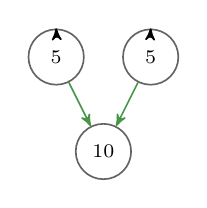
\begin{tikzpicture}[->,semithick,>=stealth',scale=1.2]
    \tikzstyle{node}=[draw=node_gray, circle, minimum size=2.0em, fill=none,text=black]
    \tikzstyle{cone}=[draw=black, circle, minimum size=1.0em, fill=none,text=black]

    \node[node] (a)  at (-0.5,0.8)  {\scriptsize $5$};
    \node[node] (b)  at (0.5,0.8)   {\scriptsize $5$};
    \node[node] (c)  at (0,-0.2)    {\scriptsize $10$};
    \path
     (-0.5,1.1) edge[] (a)
     ( 0.5,1.1) edge[] (b)
     (a) edge[edge_green] (c)
     (b) edge[edge_green] (c)
     ;
  \end{tikzpicture}
 &
  \centering
  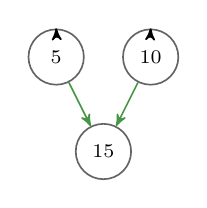
\begin{tikzpicture}[->,semithick,>=stealth',scale=1.2]
    \tikzstyle{node}=[draw=node_gray, circle, minimum size=2.0em, fill=none,text=black]
    \tikzstyle{cone}=[draw=black, circle, minimum size=1.0em, fill=none,text=black]

    \node[node] (a)  at (-0.5,0.8)  {\scriptsize $5$};
    \node[node] (b)  at (0.5,0.8)   {\scriptsize $10$};
    \node[node] (c)  at (0,-0.2)    {\scriptsize $15$};
    \path
     (-0.5,1.1) edge[] (a)
     ( 0.5,1.1) edge[] (b)
     (a) edge[edge_green] (c)
     (b) edge[edge_green] (c)
     ;
  \end{tikzpicture}
%  &
%   \begin{tikzpicture}[->,semithick,>=stealth',scale=1.2]
%     \tikzstyle{node}=[draw=node_gray, circle, minimum size=2.0em, fill=none,text=black]
%     \tikzstyle{cone}=[draw=black, circle, minimum size=1.0em, fill=none,text=black]
% 
%     \node[node] (a)  at (-0.5,0.8)  {\scriptsize $10$};
%     \node[node] (b)  at (0.5,0.8)   {\scriptsize $10$};  
%     \node[node] (c)  at (0,-0.2)    {\scriptsize $20$};
%     \path
%      (-0.5,1.1) edge[] (a)
%      ( 0.5,1.1) edge[] (b)
%      (a) edge[edge_green] (c)
%      (b) edge[edge_green] (c)
%      ;
%   \end{tikzpicture}
\end{tabular}
\caption{Five quantitative stable states of a variable with two independent regulations.}
\label{fig:or_states}
\end{figure}


\begin{figure}
\centering
\begin{tabular}{cccccc}
 $S_1\rightsquigarrow S_1$ & $S_1\rightsquigarrow S_2 $ & $S_1\rightsquigarrow S_4$
 &  $S_3\rightsquigarrow \tilde{S}_5 $ &  $S_5\rightsquigarrow \tilde{S}_5 $ &  $S_5\rightsquigarrow \tilde{S}_3 $  \\
\\                      
 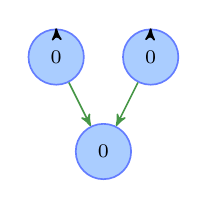
\begin{tikzpicture}[->,semithick,>=stealth',scale=1.2]
    \tikzstyle{node}=[draw=node_gray, circle, minimum size=2.0em, fill=none,text=black]
    \tikzstyle{up}=[style=node,text=black,text opacity=1,fill=node_green,draw=edge_green]
    \tikzstyle{dn}=[style=node,text=black,text opacity=1,fill=node_red,draw=edge_red]
    \tikzstyle{zn}=[style=node,text=black,text opacity=1,fill=node_blue,draw=edge_blue]
    \tikzstyle{cone}=[draw=black, circle, minimum size=1.0em, fill=none,text=black]

    \node[zn] (a)  at (-0.5,0.8)  {\scriptsize $0$};
    \node[zn] (b)  at (0.5,0.8)   {\scriptsize $0$}; 
    \node[zn] (c)  at (0,-0.2)    {\scriptsize $0$};
    \path
     (-0.5,1.1) edge[] (a)
     ( 0.5,1.1) edge[] (b)
     (a) edge[edge_green] (c)
     (b) edge[edge_green] (c)
     ;
  \end{tikzpicture}
 &
  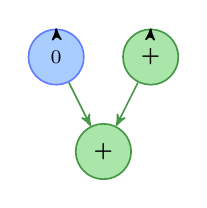
\begin{tikzpicture}[->,semithick,>=stealth',scale=1.2]
    \tikzstyle{node}=[draw=node_gray, circle, minimum size=2.0em, fill=none,text=black]
    \tikzstyle{up}=[style=node,text=black,text opacity=1,fill=node_green,draw=edge_green]
    \tikzstyle{dn}=[style=node,text=black,text opacity=1,fill=node_red,draw=edge_red]
    \tikzstyle{zn}=[style=node,text=black,text opacity=1,fill=node_blue,draw=edge_blue]
    \tikzstyle{cone}=[draw=black, circle, minimum size=1.0em, fill=none,text=black]

    \node[zn] (a)  at (-0.5,0.8)  {\scriptsize $0$};
    \node[up] (b)  at (0.5,0.8)   {\scriptsize $\plus$};
    \node[up] (c)  at (0,-0.2)    {\scriptsize $\plus$};
    \path
     (-0.5,1.1) edge[] (a)
     ( 0.5,1.1) edge[] (b)
     (a) edge[edge_green] (c)
     (b) edge[edge_green] (c)
     ;
  \end{tikzpicture}
 &
  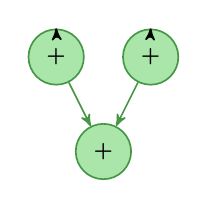
\begin{tikzpicture}[->,semithick,>=stealth',scale=1.2]
    \tikzstyle{node}=[draw=node_gray, circle, minimum size=2.0em, fill=none,text=black]
    \tikzstyle{up}=[style=node,text=black,text opacity=1,fill=node_green,draw=edge_green]
    \tikzstyle{dn}=[style=node,text=black,text opacity=1,fill=node_red,draw=edge_red]
    \tikzstyle{zn}=[style=node,text=black,text opacity=1,fill=node_blue,draw=edge_blue]
    \tikzstyle{cone}=[draw=black, circle, minimum size=1.0em, fill=none,text=black]

    \node[up] (a)  at (-0.5,0.8)  {\scriptsize $\plus$};
    \node[up] (b)  at (0.5,0.8)   {\scriptsize $\plus$};
    \node[up] (c)  at (0,-0.2)    {\scriptsize $\plus$};
    \path
     (-0.5,1.1) edge[] (a)
     ( 0.5,1.1) edge[] (b)
     (a) edge[edge_green] (c)
     (b) edge[edge_green] (c)
     ;
  \end{tikzpicture}
 &
  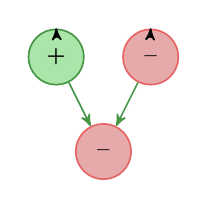
\begin{tikzpicture}[->,semithick,>=stealth',scale=1.2]
    \tikzstyle{node}=[draw=node_gray, circle, minimum size=2.0em, fill=none,text=black]
    \tikzstyle{up}=[style=node,text=black,text opacity=1,fill=node_green,draw=edge_green]
    \tikzstyle{dn}=[style=node,text=black,text opacity=1,fill=node_red,draw=edge_red]
    \tikzstyle{zn}=[style=node,text=black,text opacity=1,fill=node_blue,draw=edge_blue]
    \tikzstyle{am}=[style=node,text=black,text opacity=1,fill=node_yell,draw=edge_blue]
    \tikzstyle{cone}=[draw=black, circle, minimum size=1.0em, fill=none,text=black]


    \node[up] (a)  at (-0.5,0.8)  {\scriptsize $\plus$};
    \node[dn] (b)  at (0.5,0.8)   {\scriptsize $\minus$};  
    \node[dn] (c)  at (0,-0.2)    {\scriptsize $\minus$};
%     \node[label] (cl)  at (0.0,-0.5)  {\tiny $\minus~0~\plus$};
    \path
     (-0.5,1.1) edge[] (a)
     ( 0.5,1.1) edge[] (b)
     (a) edge[edge_green] (c)
     (b) edge[edge_green] (c)
     ;
  \end{tikzpicture} &
  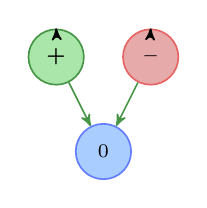
\begin{tikzpicture}[->,semithick,>=stealth',scale=1.2]
    \tikzstyle{node}=[draw=node_gray, circle, minimum size=2.0em, fill=none,text=black]
    \tikzstyle{up}=[style=node,text=black,text opacity=1,fill=node_green,draw=edge_green]
    \tikzstyle{dn}=[style=node,text=black,text opacity=1,fill=node_red,draw=edge_red]
    \tikzstyle{zn}=[style=node,text=black,text opacity=1,fill=node_blue,draw=edge_blue]
%     \tikzstyle{am}=[style=node,text=black,text opacity=1,fill=node_yell,draw=edge_blue]
    \tikzstyle{cone}=[draw=black, circle, minimum size=1.0em, fill=none,text=black]


    \node[up] (a)  at (-0.5,0.8)  {\scriptsize $\plus$};
    \node[dn] (b)  at (0.5,0.8)   {\scriptsize $\minus$};
    \node[zn] (c)  at (0,-0.2)    {\scriptsize 0};
    \path
     (-0.5,1.1) edge[] (a)
     ( 0.5,1.1) edge[] (b)
     (a) edge[edge_green] (c)
     (b) edge[edge_green] (c)
     ;
  \end{tikzpicture} &
  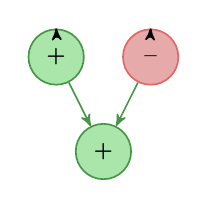
\begin{tikzpicture}[->,semithick,>=stealth',scale=1.2]
    \tikzstyle{node}=[draw=node_gray, circle, minimum size=2.0em, fill=none,text=black]
    \tikzstyle{up}=[style=node,text=black,text opacity=1,fill=node_green,draw=edge_green]
    \tikzstyle{dn}=[style=node,text=black,text opacity=1,fill=node_red,draw=edge_red]
    \tikzstyle{zn}=[style=node,text=black,text opacity=1,fill=node_blue,draw=edge_blue]
    \tikzstyle{am}=[style=node,text=black,text opacity=1,fill=node_yell,draw=edge_blue]
    \tikzstyle{cone}=[draw=black, circle, minimum size=1.0em, fill=none,text=black]


    \node[up] (a)  at (-0.5,0.8)  {\scriptsize $\plus$};
    \node[dn] (b)  at (0.5,0.8)   {\scriptsize $\minus$};
    \node[up] (c)  at (0,-0.2)    {\scriptsize $\plus$};
    \path
     (-0.5,1.1) edge[] (a)
     ( 0.5,1.1) edge[] (b)
     (a) edge[edge_green] (c)
     (b) edge[edge_green] (c)
     ;
  \end{tikzpicture}
 \\  
 \\
 a) & b) & c) & d) & e) & f)
\end{tabular}
\caption{Sign labeling representation of possible transitions among the states in Figure~\ref{fig:or_states}.
The $\sim$ means that the values of the input nodes have been switched left to right in the state.}
\label{fig:or_shifts}
\end{figure}

Figure~\ref{fig:or_states} shows exemplary five quantitative representations of stable states of 
 a system where one variable is independently regulated by two predecessors.
In Figure~\ref{fig:or_shifts} we see the possible sign labelings representing different state transitions.
We see that for the cases $a$-$c$ there exists an unambiguous input output behavior.
In the cases $d$-$f$ we see different outputs for the same input.
This behavior is implemented by the following forward propagation rule.
%
\begin{srule}\label{rule_fw}{\bf (forward propagation)} 0-change can only occur in a variable that does not depend on other variables with change, 
 or if it receives opposing regulations.

Let $(V,E,\sigma)$ be an IG.
Then a labeling $\mu : V \rightarrow \{\plus,\minus,0\}$ satisfies Rule~\ref{rule_fw} for node $i \in V$
 iff
 \begin{itemize}
  \item $\mu(i) \neq 0$, or
  \item there is no edge $j \rightarrow i$ in~$E$ such that $\mu(j)\sigma(j,i) \in \{\plus,\minus\}$, or
  \item there exist at least two edges $j_1 \rightarrow i$ and $j_2 \rightarrow i$ in~$E$
 such that $\mu(j_1)\sigma(j_1,i) + \mu(j_2)\sigma(j_2,i) = 0$. 
 \end{itemize}
\end{srule}

This rule implements forward propagation by restricting the occurrence of $0$.
In other words Rule~\ref{rule_fw} limits the cases were a change in an upstream node can have no effect
 on the regulated down stream node.
We can see now that labeling $\mu_1$ in Figure~\ref{fig:weak_prop} does not satisfy Rule~\ref{rule_fw} for $c$.
Only labeling $\mu_2$ satisfies both Rule~\ref{rule_bw} and~\ref{rule_fw} for all nodes, 
 leaving us with only one possible behavior.
 
 
\section*{Conclusion} 

In this part I have introduced the forward propagation rule for independent regulations, and
we have seen how forward propagation increases the predictive power of sign consistency methods.
In the next part I will show how we can implement forward propagation for cooperative (dependent) regulations.


\chapter*{Predicting effects on cooperatively regulated variables}
\addcontentsline{toc}{chapter}{Predicting effects on cooperatively regulated variables}
The previous part introduced the forward propagation rule for independent regulations.
I mentioned that there exists a second kind of regulations, cooperative dependent regulation.
While for independent regulation $i \rightarrow j$  a change in $i$ is sufficient to cause an change in $j$,
it depends for cooperative regulations on multiple variables whether the change in $i$ will have an effect on $j$.
Cooperative regulation exists in various forms in biological systems as chemical reactions that need multiple reactants or complex protein interactions.
In this part I will show how cooperative regulations can be modeled within the sign consistency approach.


\section*{Forward propagation in cooperatively regulated variables}

Cooperative regulations are represented as distinct type of variables in our system
 similiar to {\bf AND} nodes of a logic network.
The basic idea behind cooperative regulation is that one needs all regulators to have an effect, 
 but there exist only one limiting factor.
It might be sufficient to increase (resp. decrease) one of the regulators to change the limiting factor, but
to ensure a change in the limiting factor all regulators have to increase (resp. decrease).

\begin{figure}
\begin{tabular}{p{65pt}p{65pt}p{65pt}p{65pt}p{65pt}}
 \centering $S_1$ & \centering $S_2$ & \centering $S_3$ & \centering $S_4$ & \centering $S_5$ % & $S_6$
 \cr &
 \\
  \centering
  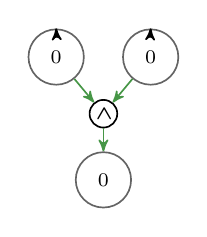
\begin{tikzpicture}[->,semithick,>=stealth',scale=1.2]
    \tikzstyle{node}=[draw=node_gray, circle, minimum size=2.0em, fill=none,text=black]
    \tikzstyle{cone}=[draw=black, circle, minimum size=1.0em, fill=none,text=black]

    \node[node] (a)  at (-0.5,0.8)  {\scriptsize $0$};
    \node[node] (b)  at (0.5,0.8)   {\scriptsize $0$};
    \node[cone] (op) at (0,0.2)     {};                 \node[] (l) at (0.01,0.2)  {\scriptsize $\boldsymbol{ \wedge}$};
    \node[node] (c)  at (0,-0.5)    {\scriptsize $0$};
    \path
     (-0.5,1.1) edge[] (a)
     ( 0.5,1.1) edge[] (b)
     (a)  edge[edge_green] (op)
     (b)  edge[edge_green] (op)
     (op) edge[edge_green] (c)
     ;
  \end{tikzpicture}
 &  
  \centering
  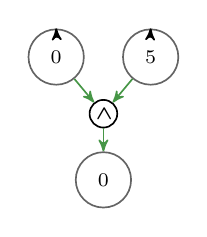
\begin{tikzpicture}[->,semithick,>=stealth',scale=1.2]
    \tikzstyle{node}=[draw=node_gray, circle, minimum size=2.0em, fill=none,text=black]
    \tikzstyle{cone}=[draw=black, circle, minimum size=1.0em, fill=none,text=black]

    \node[node] (a)  at (-0.5,0.8)  {\scriptsize $0$};
    \node[node] (b)  at (0.5,0.8)   {\scriptsize $5$};
    \node[cone] (op) at (0,0.2)     {};                 \node[] (l) at (0.01,0.2)  {\scriptsize $\boldsymbol{ \wedge}$};    
    \node[node] (c)  at (0,-0.5)    {\scriptsize $0$};
    \path
     (-0.5,1.1) edge[] (a)
     ( 0.5,1.1) edge[] (b)
     (a)  edge[edge_green] (op)
     (b)  edge[edge_green] (op)
     (op) edge[edge_green] (c)
     ;
  \end{tikzpicture}
 &
  \centering
  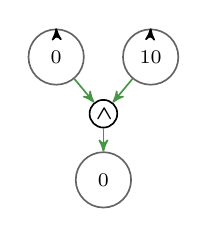
\begin{tikzpicture}[->,semithick,>=stealth',scale=1.2]
    \tikzstyle{node}=[draw=node_gray, circle, minimum size=2.0em, fill=none,text=black]
    \tikzstyle{cone}=[draw=black, circle, minimum size=1.0em, fill=none,text=black]

    \node[node] (a)  at (-0.5,0.8)  {\scriptsize $0$};
    \node[node] (b)  at (0.5,0.8)   {\scriptsize $10$};
    \node[cone] (op) at (0,0.2)     {};                 \node[] (l) at (0.01,0.2)  {\scriptsize $\boldsymbol{ \wedge}$};    
    \node[node] (c)  at (0,-0.5)    {\scriptsize $0$};
    \path
     (-0.5,1.1) edge[] (a)
     ( 0.5,1.1) edge[] (b)
     (a)  edge[edge_green] (op)
     (b)  edge[edge_green] (op)
     (op) edge[edge_green] (c)
     ;
  \end{tikzpicture}
 &
  \centering
  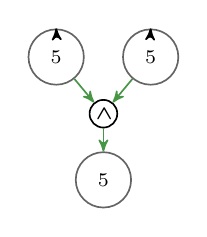
\begin{tikzpicture}[->,semithick,>=stealth',scale=1.2]
    \tikzstyle{node}=[draw=node_gray, circle, minimum size=2.0em, fill=none,text=black]
    \tikzstyle{cone}=[draw=black, circle, minimum size=1.0em, fill=none,text=black]

    \node[node] (a)  at (-0.5,0.8)  {\scriptsize $5$};
    \node[node] (b)  at (0.5,0.8)   {\scriptsize $5$};
    \node[cone] (op) at (0,0.2)     {};                 \node[] (l) at (0.01,0.2)  {\scriptsize $\boldsymbol{ \wedge}$};    
    \node[node] (c)  at (0,-0.5)    {\scriptsize $5$};
    \path
     (-0.5,1.1) edge[] (a)
     ( 0.5,1.1) edge[] (b)
     (a)  edge[edge_green] (op)
     (b)  edge[edge_green] (op)
     (op) edge[edge_green] (c)
     ;
  \end{tikzpicture}
 &
  \centering
  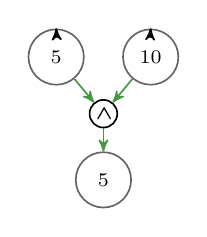
\begin{tikzpicture}[->,semithick,>=stealth',scale=1.2]
    \tikzstyle{node}=[draw=node_gray, circle, minimum size=2.0em, fill=none,text=black]
    \tikzstyle{cone}=[draw=black, circle, minimum size=1.0em, fill=none,text=black]

    \node[node] (a)  at (-0.5,0.8)  {\scriptsize $5$};
    \node[node] (b)  at (0.5,0.8)   {\scriptsize $10$};
    \node[cone] (op) at (0,0.2)     {};                 \node[] (l) at (0.01,0.2)  {\scriptsize $\boldsymbol{ \wedge}$};    
    \node[node] (c)  at (0,-0.5)    {\scriptsize $5$};
    \path
     (-0.5,1.1) edge[] (a)
     ( 0.5,1.1) edge[] (b)
     (a)  edge[edge_green] (op)
     (b)  edge[edge_green] (op)
     (op) edge[edge_green] (c)
     ;
  \end{tikzpicture}
%  &
%   \begin{tikzpicture}[->,semithick,>=stealth',scale=1.2]
%     \tikzstyle{node}=[draw=node_gray, circle, minimum size=2.0em, fill=none,text=black]
%     \tikzstyle{cone}=[draw=black, circle, minimum size=1.0em, fill=none,text=black]
% 
%     \node[node] (a)  at (-0.5,0.8)  {\scriptsize $10$};
%     \node[node] (b)  at (0.5,0.8)   {\scriptsize $10$};
%     \node[cone] (op) at (0,0.2)     {};                 \node[] (l) at (0.01,0.2)  {\scriptsize $\boldsymbol{ \wedge}$};    
%     \node[node] (c)  at (0,-0.5)    {\scriptsize $10$};
%     \path
%      (-0.5,1.1) edge[] (a)
%      ( 0.5,1.1) edge[] (b)
%      (a)  edge[edge_green] (op)
%      (b)  edge[edge_green] (op)
%      (op) edge[edge_green] (c)
%      ;
%   \end{tikzpicture}
\end{tabular}
\caption{Five quantitative stable states of a cooperatively regulated variable.}
\label{fig:and_states}
\end{figure}



\begin{figure}
\centering
\begin{tabular}{ccccccc}
 $S_1\rightsquigarrow S_1$ & $S_1\rightsquigarrow S_2$ & $\tilde{S}_2\rightsquigarrow S_4$ & $S_1\rightsquigarrow S_4$ & $S_5\rightsquigarrow \tilde{S}_3$ 
 & $S_5\rightsquigarrow \tilde{S}_5$ & $S_3\rightsquigarrow \tilde{S}_5$  \\
\\                          
 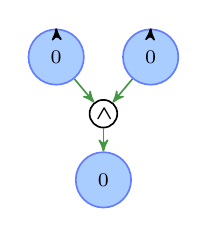
\begin{tikzpicture}[->,semithick,>=stealth',scale=1.2]
    \tikzstyle{node}=[draw=node_gray, circle, minimum size=2.0em, fill=none,text=black]
    \tikzstyle{up}=[style=node,text=black,text opacity=1,fill=node_green,draw=edge_green]
    \tikzstyle{dn}=[style=node,text=black,text opacity=1,fill=node_red,draw=edge_red]
    \tikzstyle{zn}=[style=node,text=black,text opacity=1,fill=node_blue,draw=edge_blue]
    \tikzstyle{cone}=[draw=black, circle, minimum size=1.0em, fill=none,text=black]

    \node[zn] (a)  at (-0.5,0.8)  {\scriptsize $0$};
    \node[zn] (b)  at (0.5,0.8)   {\scriptsize $0$};
    \node[cone] (op) at (0,0.2)     {};                 \node[] (l) at (0.01,0.2)  {\scriptsize $\boldsymbol{ \wedge}$};    
    \node[zn] (c)  at (0,-0.5)    {\scriptsize $0$};
    \path
     (-0.5,1.1) edge[] (a)
     ( 0.5,1.1) edge[] (b)
     (a)  edge[edge_green] (op)
     (b)  edge[edge_green] (op)
     (op) edge[edge_green] (c)
     ;
  \end{tikzpicture}
 &
  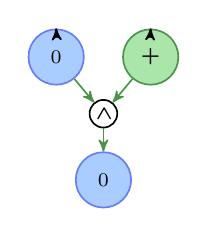
\begin{tikzpicture}[->,semithick,>=stealth',scale=1.2]
    \tikzstyle{node}=[draw=node_gray, circle, minimum size=2.0em, fill=none,text=black]
    \tikzstyle{up}=[style=node,text=black,text opacity=1,fill=node_green,draw=edge_green]
    \tikzstyle{dn}=[style=node,text=black,text opacity=1,fill=node_red,draw=edge_red]
    \tikzstyle{zn}=[style=node,text=black,text opacity=1,fill=node_blue,draw=edge_blue]
    \tikzstyle{cone}=[draw=black, circle, minimum size=1.0em, fill=none,text=black]

    \node[zn] (a)  at (-0.5,0.8)  {\scriptsize $0$};
    \node[up] (b)  at (0.5,0.8)   {\scriptsize $\plus$};
    \node[cone] (op) at (0,0.2)     {};                 \node[] (l) at (0.01,0.2)  {\scriptsize $\boldsymbol{ \wedge}$};    
    \node[zn] (c)  at (0,-0.5)    {\scriptsize 0};
%     \node[]     (cl) at (0.0,-0.5)  {\scriptsize $0 ~ \plus$};
    \path
     (-0.5,1.1) edge[] (a)
     ( 0.5,1.1) edge[] (b)
     (a)  edge[edge_green] (op)
     (b)  edge[edge_green] (op)
     (op) edge[edge_green] (c)
     ;
  \end{tikzpicture}
 &
  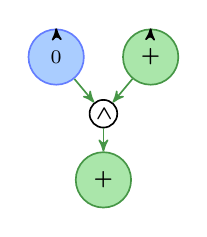
\begin{tikzpicture}[->,semithick,>=stealth',scale=1.2]
    \tikzstyle{node}=[draw=node_gray, circle, minimum size=2.0em, fill=none,text=black]
    \tikzstyle{up}=[style=node,text=black,text opacity=1,fill=node_green,draw=edge_green]
    \tikzstyle{dn}=[style=node,text=black,text opacity=1,fill=node_red,draw=edge_red]
    \tikzstyle{zn}=[style=node,text=black,text opacity=1,fill=node_blue,draw=edge_blue]
    \tikzstyle{cone}=[draw=black, circle, minimum size=1.0em, fill=none,text=black]

    \node[zn] (a)  at (-0.5,0.8)  {\scriptsize $0$};
    \node[up] (b)  at (0.5,0.8)   {\scriptsize $\plus$};
    \node[cone] (op) at (0,0.2)     {};                 \node[] (l) at (0.01,0.2)  {\scriptsize $\boldsymbol{ \wedge}$};    
    \node[up] (c)  at (0,-0.5)    {\scriptsize $\plus$};
%     \node[]     (cl) at (0.0,-0.5)  {\scriptsize $0 ~ \plus$};
    \path
     (-0.5,1.1) edge[] (a)
     ( 0.5,1.1) edge[] (b)
     (a)  edge[edge_green] (op)
     (b)  edge[edge_green] (op)
     (op) edge[edge_green] (c)
     ;
  \end{tikzpicture}
 &
  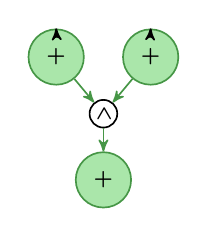
\begin{tikzpicture}[->,semithick,>=stealth',scale=1.2]
    \tikzstyle{node}=[draw=node_gray, circle, minimum size=2.0em, fill=none,text=black]
    \tikzstyle{up}=[style=node,text=black,text opacity=1,fill=node_green,draw=edge_green]
    \tikzstyle{dn}=[style=node,text=black,text opacity=1,fill=node_red,draw=edge_red]
    \tikzstyle{zn}=[style=node,text=black,text opacity=1,fill=node_blue,draw=edge_blue]
    \tikzstyle{cone}=[draw=black, circle, minimum size=1.0em, fill=none,text=black]

    \node[up] (a)  at (-0.5,0.8)  {\scriptsize $\plus$};
    \node[up] (b)  at (0.5,0.8)   {\scriptsize $\plus$};
    \node[cone] (op) at (0,0.2)     {};                 \node[] (l) at (0.01,0.2)  {\scriptsize $\boldsymbol{ \wedge}$};    
    \node[up] (c)  at (0,-0.5)    {\scriptsize $\plus$};
    \path
     (-0.5,1.1) edge[] (a)
     ( 0.5,1.1) edge[] (b)
     (a)  edge[edge_green] (op)
     (b)  edge[edge_green] (op)
     (op) edge[edge_green] (c)
     ;
  \end{tikzpicture}
 &
  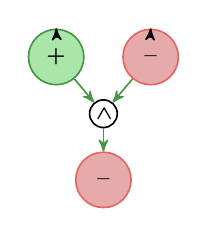
\begin{tikzpicture}[->,semithick,>=stealth',scale=1.2]
    \tikzstyle{node}=[draw=node_gray, circle, minimum size=2.0em, fill=none,text=black]
    \tikzstyle{up}=[style=node,text=black,text opacity=1,fill=node_green,draw=edge_green]
    \tikzstyle{dn}=[style=node,text=black,text opacity=1,fill=node_red,draw=edge_red]
    \tikzstyle{zn}=[style=node,text=black,text opacity=1,fill=node_blue,draw=edge_blue]
    \tikzstyle{cone}=[draw=black, circle, minimum size=1.0em, fill=none,text=black]

    \node[up] (a)  at (-0.5,0.8)  {\scriptsize $\plus$};
    \node[dn] (b)  at (0.5,0.8)   {\scriptsize $\minus$};
    \node[cone] (op) at (0,0.2)     {};                 \node[] (l) at (0.01,0.2)  {\scriptsize $\boldsymbol{ \wedge}$};    
    \node[dn] (c)  at (0,-0.5)    {\scriptsize $\minus$};
%     \node[]     (cl) at (0.0,-0.5)  {\tiny $\minus~0~\plus$};
    \path
     (-0.5,1.1) edge[] (a)
     ( 0.5,1.1) edge[] (b)
     (a)  edge[edge_green] (op)
     (b)  edge[edge_green] (op)
     (op) edge[edge_green] (c)
     ;
  \end{tikzpicture}
 &
  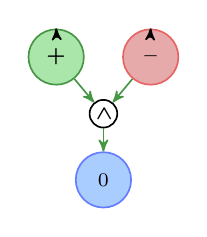
\begin{tikzpicture}[->,semithick,>=stealth',scale=1.2]
    \tikzstyle{node}=[draw=node_gray, circle, minimum size=2.0em, fill=none,text=black]
    \tikzstyle{up}=[style=node,text=black,text opacity=1,fill=node_green,draw=edge_green]
    \tikzstyle{dn}=[style=node,text=black,text opacity=1,fill=node_red,draw=edge_red]
    \tikzstyle{zn}=[style=node,text=black,text opacity=1,fill=node_blue,draw=edge_blue]
    \tikzstyle{cone}=[draw=black, circle, minimum size=1.0em, fill=none,text=black]

    \node[up] (a)  at (-0.5,0.8)  {\scriptsize $\plus$};
    \node[dn] (b)  at (0.5,0.8)   {\scriptsize $\minus$};
    \node[cone] (op) at (0,0.2)     {};                 \node[] (l) at (0.01,0.2)  {\scriptsize $\boldsymbol{ \wedge}$};    
    \node[zn] (c)  at (0,-0.5)    {\scriptsize 0};
%     \node[]     (cl) at (0.0,-0.5)  {\tiny $\minus~0~\plus$};
    \path
     (-0.5,1.1) edge[] (a)
     ( 0.5,1.1) edge[] (b)
     (a)  edge[edge_green] (op)
     (b)  edge[edge_green] (op)
     (op) edge[edge_green] (c)
     ;
  \end{tikzpicture}
 &
  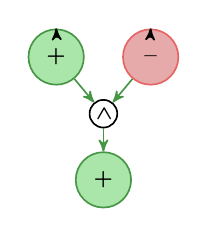
\begin{tikzpicture}[->,semithick,>=stealth',scale=1.2]
    \tikzstyle{node}=[draw=node_gray, circle, minimum size=2.0em, fill=none,text=black]
    \tikzstyle{up}=[style=node,text=black,text opacity=1,fill=node_green,draw=edge_green]
    \tikzstyle{dn}=[style=node,text=black,text opacity=1,fill=node_red,draw=edge_red]
    \tikzstyle{zn}=[style=node,text=black,text opacity=1,fill=node_blue,draw=edge_blue]
    \tikzstyle{cone}=[draw=black, circle, minimum size=1.0em, fill=none,text=black]

    \node[up] (a)  at (-0.5,0.8)  {\scriptsize $\plus$};
    \node[dn] (b)  at (0.5,0.8)   {\scriptsize $\minus$};
    \node[cone] (op) at (0,0.2)     {};                 \node[] (l) at (0.01,0.2)  {\scriptsize $\boldsymbol{ \wedge}$};    
    \node[up] (c)  at (0,-0.5)    {\scriptsize $\plus$};
%     \node[]     (cl) at (0.0,-0.5)  {\tiny $\minus~0~\plus$};
    \path
     (-0.5,1.1) edge[] (a)
     ( 0.5,1.1) edge[] (b)
     (a)  edge[edge_green] (op)
     (b)  edge[edge_green] (op)
     (op) edge[edge_green] (c)
     ;
  \end{tikzpicture}
  \\
  \\
   a) & b) & c) & d) & e) & f) & g)
\end{tabular}
\caption{Sign labeling representation of possible transitions among the states in Figure~\ref{fig:and_states}.
The $\sim$ means that the values of the input nodes have been switched left to right in the state.}
\label{fig:and_shifts}
\end{figure}

Figure~\ref{fig:and_states} shows exemplarily five quantitative representations of stable states of 
 a system were one variable is cooperatively regulated by two predecessors.
In Figure~\ref{fig:and_shifts} we see the possible sign labelings representing different state transitions.
%
We see that for the cases $a$ and $d$ there exists an unambiguous input output behavior.
In the cases $b$-$c$ and $e$-$g$ we see different outputs for the same input.
In both state transistions $b$ and $c$ we have an increase in one of the regulators while the other regulator remains unchanged,
 but only in $c$ the limiting factor has changed leading to a change in the regulated variable.
This behavior is implemented by the following forward propagation rule.
%
\begin{srule}\label{rule_fw_coop}{\bf (forward propagation cooperative regulation)} 0-change can only occur in a variable that depends on a another variable that shows 0-change
 or if it receives opposing regulations.

Let $(V,E,\sigma)$ be an IG and $V_C \subseteq V$ cooperatively regulated variables.
Then a labeling $\mu : V \rightarrow \{\plus,\minus,0\}$ satisfies Rule~\ref{rule_fw_coop} for node $i \in V_C$
 iff
 \begin{itemize}
  \item $\mu(i) \neq 0$, or
  \item there is no edge $j \rightarrow i$ in~$E$ such that $\mu(j)\sigma(j,i) \in \{\plus,\minus\}$, or
  \item there is an edge $j \rightarrow i$ in~$E$ such that $\sigma(j,i)= 0$, or
  \item there exist at least two edges $j_1 {\,\rightarrow\,} i$ and $j_2 {\,\rightarrow\,} i$ in~$E$
 such that $\mu(j_1)\sigma(j_1,i) + \mu(j_2)\sigma(j_2,i) = 0$. 
 \end{itemize}
\end{srule}
This rule implements forward propagation by restricting the occurrence of $0$.
In other words Rule~\ref{rule_fw_coop} limits the cases were a change in an upstream node can have no effect
 on the regulated down stream node.

\section*{Conclusion} 

In this part I introduced the forward propagation rule for cooperative regulations.
In the next part I will introduce a consistency rule that allow us to filter unfounded self regulations.

\chapter*{Excluding circular self regulation}
\addcontentsline{toc}{chapter}{Excluding circular self regulation}
In this part I will introduce a new global consistency rule to ensure that every change
is justified by a chain of influences that can be traced back to an input node.
This natural constraint is especially useful to exclude self-justification of changes via positive feedback loops.


\section*{Circular regulation}

In most biological systems we find circular regulation via feedback loops.
For the consistency rules that we've covered so far circular regulations pose the problem that
 they allow to represent state transistions for which we can not identify the reason that trigger the state change.
For example in Figure~\ref{fig:founded} we see an IG with labelings that explain an increase in $d$.
Both total labelings satisfy the propagation rules (Rule~\ref{rule_bw} and~\ref{rule_fw}).
For $\mu_1$ we see a circular up regulation in $b$ and $c$, which is used as explanation for the increase in $d$,
 but we don't know why $b$ and $c$ have increase in the first place.
Only the labeling $\mu_{2}$ allows us to identify a trigger for the state change, i.e. the increase in $a$.

\begin{figure}
\small
\centering
\begin{tabular}{p{70pt}p{70pt}p{70pt}p{70pt}}
  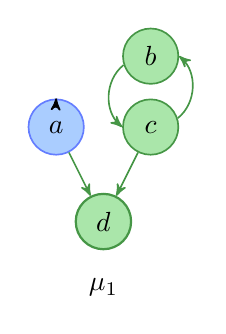
\begin{tikzpicture}[->,semithick,>=stealth',scale=1.2]
    \tikzstyle{label}=[text=black] 
    \tikzstyle{node}=[draw=node_gray, circle, minimum size=2.0em, fill=none,text=black]
    \tikzstyle{up}=[style=node,text=black,text opacity=1,fill=node_green,draw=edge_green]
    \tikzstyle{dn}=[style=node,text=black,text opacity=1,fill=node_red,draw=edge_red]
    \tikzstyle{zn}=[style=node,text=black,text opacity=1,fill=node_blue,draw=edge_blue]
    \node[zn] (A) at (0.5,1)    {$a$};
    \node[up] (B) at (1.5,1)    {$c$};
    \node[up] (C) at (1.5,1.75) {$b$};
    \node[up,thick] (D) at (1,0)      {$d$};
    \node[label] (l1) at (1,-0.7) {$\mu_1$};
    
    \path[every node/.style={anchor=south}]
     (0.5,1.3) edge[] (A)
     (A) edge[edge_green] (D)
     (B) edge[edge_green,bend right=50] (C.east)
     (C) edge[edge_green,bend right=50] (B.west)     
     (B) edge[edge_green] (D);
  \end{tikzpicture}
%   &
%   \begin{tikzpicture}[->,semithick,>=stealth',scale=1.2]
%     \tikzstyle{label}=[text=black] 
%     \tikzstyle{node}=[draw=node_gray, circle, minimum size=2.0em, fill=none,text=black]
%     \tikzstyle{up}=[style=node,text=black,text opacity=1,fill=node_green,draw=edge_green]
%     \tikzstyle{dn}=[style=node,text=black,text opacity=1,fill=node_red,draw=edge_red]
%     \tikzstyle{zn}=[style=node,text=black,text opacity=1,fill=node_blue,draw=edge_blue]
%     \node[up] (A) at (0.5,1)    {$a$};
%     \node[dn] (B) at (1.5,1)    {$c$};
%     \node[dn] (C) at (1.5,1.75) {$b$};
%     \node[up,thick] (D) at (1,0)      {$d$};   
%     \node[label] (l1) at (1,-0.7) {$\mu_2$};
%     
%     \path[every node/.style={anchor=south}]
%      (0.5,1.3) edge[] (A)
%      (A) edge[edge_green] (D)
%      (B) edge[edge_green,bend right=50] (C.east)
%      (C) edge[edge_green,bend right=50] (B.west)     
%      (B) edge[edge_green] (D);
%   \end{tikzpicture}
  & 
  \begin{tikzpicture}[->,semithick,>=stealth',scale=1.2]
    \tikzstyle{label}=[text=black] 
    \tikzstyle{node}=[draw=node_gray, circle, minimum size=2.0em, fill=none,text=black]
    \tikzstyle{up}=[style=node,text=black,text opacity=1,fill=node_green,draw=edge_green]
    \tikzstyle{dn}=[style=node,text=black,text opacity=1,fill=node_red,draw=edge_red]
    \tikzstyle{zn}=[style=node,text=black,text opacity=1,fill=node_blue,draw=edge_blue]

    \node[up] (A) at (0.5,1)    {$a$};
    \node[zn] (B) at (1.5,1)    {$c$};
    \node[zn] (C) at (1.5,1.75) {$b$};
    \node[up,thick] (D) at (1,0)      {$d$};
    \node[label] (l1) at (1,-0.7) {$\mu_2$};
    
    \path[every node/.style={anchor=south}]
     (0.5,1.3) edge[] (A)
     (A) edge[edge_green] (D)
     (B) edge[edge_green,bend right=50] (C.east)
     (C) edge[edge_green,bend right=50] (B.west)     
     (B) edge[edge_green] (D);
  \end{tikzpicture}
%   &
%   \begin{tikzpicture}[->,semithick,>=stealth',scale=1.2]
%     \tikzstyle{label}=[text=black] 
%     \tikzstyle{node}=[draw=node_gray, circle, minimum size=2.0em, fill=none,text=black]
%     \tikzstyle{up}=[style=node,text=black,text opacity=1,fill=node_green,draw=edge_green]
%     \tikzstyle{dn}=[style=node,text=black,text opacity=1,fill=node_red,draw=edge_red]
%     \tikzstyle{zn}=[style=node,text=black,text opacity=1,fill=node_blue,draw=edge_blue]
% 
%     \node[up] (A) at (0.5,1)    {$a$};
%     \node[up] (B) at (1.5,1)    {$c$};
%     \node[up] (C) at (1.5,1.75) {$b$};
%     \node[up,thick] (D) at (1,0)      {$d$};
%     \node[label] (l1) at (1,-0.7) {$\mu_4$};
%     
%     \path[every node/.style={anchor=south}]
%      (0.5,1.3) edge[] (A)
%      (A) edge[edge_green] (D)
%      (B) edge[edge_green,bend right=50] (C.east)
%      (C) edge[edge_green,bend right=50] (B.west)     
%      (B) edge[edge_green] (D);
%   \end{tikzpicture}
  \end{tabular}  
  \caption{Example for an influence graph with self regulation. An increase in $d$ can be 
   explained either by self activation in $b$ and $c$ or by the input node $a$.}
  \label{fig:founded}
\end{figure} 

To filter labelings which represent circular explanations we introduce the following consistency rule.
  
\begin{srule}\label{rule_founded}{\bf (a change must be founded in an input).}
Let $(V,E,\sigma)$ be an IG and $I \subseteq V$ the input nodes.
Then a labeling $\mu : V \rightarrow \{\plus,\minus,0\}$ satisfies Rule~\ref{rule_founded} for $i \in V$ if
 \begin{itemize}
  \item $i \in I$, or
  \item $\mu(i)=0$, or
  \item there exist a path $(v_0,\dots,v_k)$ in $E$ with $v_0 \in I$, $v_k=i$ and
 $\mu(v_{n-1})\sigma(v_{n-1},v_n)=\mu(v_{n})$ for all $n=1\dots k$.
 \end{itemize}
\end{srule}

Using Rule~\ref{rule_founded} we can avoid manual removal of positive
 feedback loops as done in other approaches, and identify state transitions which can be explained by external perturbations.
Only the labeling $\mu_2$ satisfies Rule~\ref{rule_founded}.
Consistency rule~\ref{rule_founded} is especially useful if we want apply sign consistency methods in the context of perturbation experiments.
When we are actually interested in the response to perturbations,
or if we want to identify possible perturbations that trigger desired state transitions.

\section*{Conclusion}

This part introduced a consistency rule that allows us to exclude unfounded self regulations.
In the next part I will show how we can relate our model to actual measurement data via sign constraints.


\chapter*{Excluding feedback regulations}
\addcontentsline{toc}{chapter}{Excluding feedback regulation}
To filter labelings which include secondary regulations over feedback loops we use the following consistency rule.
  
\begin{srule}\label{rule_elem}{\bf (a change must be founded in an input).}
Every change must be explained via an elementary path to an input.
Let $(V,E,\sigma)$ be an IG and $I \subseteq V$ the input nodes.
Then a labeling $\mu : V \rightarrow \{\plus,\minus,0\}$ satisfies Rule~\ref{rule_elem} for $i \in V$ if
 \begin{itemize}
  \item $i \in I$, or
  \item $\mu(i)=0$, or
  \item there exist an elementary path $(v_0,\dots,v_k)$ in $E$ with $v_0 \in I$, $v_k=i$ and
 $\mu(v_{n-1})\sigma(v_{n-1},v_n)=\mu(v_{n})$ for all $n=1\dots k$.
 \end{itemize}
\end{srule}


\chapter*{Model consistency wrt. measuremented data}
\addcontentsline{toc}{chapter}{Model consistency wrt. measuremented data}
In the previous parts we covered inputs and how we can reason on perturbations of the system.
In this part we will see how we can relate actual experimental measurements to our model.

\section*{Suitable experiments}

First, we have to clarify what kind of measurements can be used for our approach and the sign consistency rules we apply.
Because the sign consistency methods reasons over the changes between states,
 we need the measurements of at least two states.
% This means we deal with at least two measurements a reference experiment and an operating experiment.
Further, the measured system states have to be compatible with the sign consistency rules that we want to apply.
For example, Rule~1 reasons over steady state changes. 
This means, if we want to use Rule~1 we have to ensure that the measured states are steady states.
There exist other sign consistency rules that work under different assumptions and reason over transitional states or early responses of the system,
 in any case it must always be ensured that the measured changes satisfy the assumptions.

 
\section*{Discretization} 

If the experimental data satisfies our assumptions, we can discretize the data and compute sign constraints.
For measured variables $v \in V$,
 we compute the difference between the values measured in a reference state and an operational state $obs(v) = (v_R - v_O)$.
The result is a value in $\mathbb{R}$. 
Depending on four thresholds $t_1 \leq t_2 < 0 < t_3 \leq t_4$, that should be defined on a case by case basis,
 we can use the quantitative change to define five deiscrete observation types.
As illustrated in Figure~\ref{fig:sign_discretization}, 
these thresholds define a (partial) mapping $\nu: V \rightarrow \{ \minus, \uncertaindecrease, 0, \uncertainincrease, \plus \}$ as follows:
\[
\nu(s)=\left \{
\begin{array}{lll}
    \minus              & |\quad        & obs(s) \leq t_1, \\  
    \uncertaindecrease  & |\quad t_1 <  & obs(s) \leq t_2,\\
    0                   & |\quad t_2 <  & obs(s) < t_3, \\
    \uncertainincrease  & |\quad t_3 \leq & obs(s) < t_4,\\
    \plus               & |\quad t_4 \leq & obs(s) \\
    \bot                & |\quad else.
\end{array} \right . 
\]
%
  \begin{figure}[h!]
  \centering
  \begin{tikzpicture}[scale=1.0]

  \tikzstyle{label}=[text=black]
  \tikzstyle{species}=[minimum size=0.2ex, maximum size=0.2ex, fill=none,text=black]
  
  \shade[left color=edge_red, right color=node_red](0,0) rectangle (1,0.5);
  \shade[left color=node_red, right color=node_blue](1,0) rectangle (4,0.5);
  \shade[left color=node_blue,right color=node_green](4,0) rectangle (7,0.5);
  \shade[left color=node_green,right color=edge_green](7,0) rectangle (8,0.5);
  
  \draw[<->,semithick]  (0,0) -- (8,0);
  \draw[dashed] (1.3,-0.1) -- (1.3,0.5);
  \draw[dashed] (3.3,-0.1) -- (3.3,0.5);
  \draw[dashed] (4.7,-0.1) -- (4.7,0.5);
  \draw[dashed] (6.8,-0.1) -- (6.8,0.5);
  \node[label]  (l1) at (1.3,-0.3)  {$t_1$};
  \node[label]  (l2) at (3.3,-0.3)  {$t_2$};
  \node[label]  (l3) at (4.7,-0.3)  {$t_3$};
  \node[label]  (l4) at (6.8,-0.3)  {$t_4$};
  \node[label]  (l5) at (4,-0.3)  {$0$};
  
  \node[label]  (l1) at (0.6,1)  {~$\minus$};
  \node[label]  (l2) at (2.3,1)  {~$\uncertaindecrease$};
  \node[label]  (l3) at (4,1)  {$0$};
  \node[label]  (l4) at (5.7,1)  {~$\uncertainincrease$};
  \node[label]  (l5) at (7.4,1)  {$\plus$};
  
  \draw [decorate,decoration={brace,amplitude=5pt,raise=2pt},yshift=0pt]
  (0,0.5) -- (1.3,0.5) node [black,midway,xshift=0.8cm] {\footnotesize };
  
  \draw [decorate,decoration={brace,amplitude=5pt,raise=2pt},yshift=0pt]
  (1.3,0.5) -- (3.3,0.5) node [black,midway,xshift=0.8cm] {\footnotesize };

  \draw [decorate,decoration={brace,amplitude=5pt,raise=2pt},yshift=0pt]
  (3.3,0.5) -- (4.7,0.5) node [black,midway,xshift=0.8cm] {\footnotesize };

  \draw [decorate,decoration={brace,amplitude=5pt,raise=2pt},yshift=0pt]
  (4.7,0.5) -- (6.8,0.5) node [black,midway,xshift=0.8cm] {\footnotesize };

  \draw [decorate,decoration={brace,amplitude=5pt,raise=2pt},yshift=0pt]
  (6.8,0.5) -- (8,0.5) node [black,midway,xshift=0.8cm] {\footnotesize };
\end{tikzpicture}
  \caption{Discretization of observed changes into sign constraints.}
  \label{fig:sign_discretization}
  \end{figure} 

We consider measurements which are smaller than $t_1$, bigger than $t_4$, and between $t_2$ and $t_3$
 as certain (decrease \minus, increase \plus, no-change 0)
 while measurements that are between $t_1$ and $t_2$ (resp. $t_3$ and $t_4$) are uncertain
 (uncertain-decrease $\uncertaindecrease$, uncertain-increase $\uncertainincrease$) and not exactly classifiable. 

\section*{Consistency checking model wrt. observed changes}
 
Given an IG $(V,E,\sigma)$ 
 and observed changes $\nu$ 
 we can define the rules that restrict the possible sign labelings of the IG model s.t. they reflect the observed behavior.
% For this purpose we look for labelings $\mu: V \rightarrow \{ \minus, 0, \plus \}$ 
% that satisfy the rules defined below.
It is important to notice that we are looking for labelings $\mu_i: V \rightarrow \{ \minus, 0, \plus \}$
 using the \emph{three} sign labels $\{\minus,0,\plus\}$
 whereas $\nu$ defines an observation labeling
 based on the \emph{five} observation labels  $\{ \minus, \uncertaindecrease, 0, \uncertainincrease, \plus \}$
 representing the discretized measurements.

\begin{srule}\label{def:constraint_obs}{\bf (satisfy observations)}
Every observed change must be consistent with the labeling.

Let $(V,E,\sigma)$ be an IG, $\nu$ an observation labeling $\nu: V \rightarrow \{ \minus, \uncertaindecrease, 0, \uncertainincrease, \plus \}$
 representing observed changes in the system.
Then a labeling $\mu : V \rightarrow \{\plus,\minus,0\}$ satisfies Rule~\ref{def:constraint_obs} for node $i\in V$
 iff
 \begin{itemize}
  \item $\mu(i)=\plus$ and $\nu(i)\in \{ \plus, \uncertainincrease \}$, or
  \item $\mu(i)=0$ and $\nu(i)\in \{ \uncertainincrease, 0, \uncertaindecrease\}$, or
  \item $\mu(i)=\minus$ and $\nu(i) \in \{ \uncertaindecrease, \minus \}$, or
  \item $\nu(i)= \bot$.  
 \end{itemize}

\end{srule}
%
This rule ensures that a labeling is compatible with the measured changes.
Note, uncertain measurements restrict the labeling of a node to two out of the three values $\{\plus, \minus, 0\}$,
while measurements with high certainty fix a node's label to exactly one value.
In Figure~\ref{fig:obs_label} we see a partial observations labeling and the corresponding sign labelings 
 that satisfy Rule~\ref{def:constraint_obs}.
Note that only the labeling $\mu_{11}$ satisfies Rule~1.
This means using sign consistency we can use incomplete and uncertain measurent data to make predictions on the behavior of unobserved system variables.

\begin{figure}
\begin{tabular}{ccccc}%{p{70pt}p{60pt}p{60pt}p{60pt}p{60pt}}
  \begin{tikzpicture}[->,semithick,>=stealth',scale=1.2]
    \tikzstyle{node}=[draw=node_gray, circle, minimum size=2.0em, fill=none,text=black]
    \tikzstyle{up}=[style=node,text=black,text opacity=1,fill=node_green,draw=edge_green]
    \tikzstyle{dn}=[style=node,text=black,text opacity=1,fill=node_red,draw=edge_red]
    \tikzstyle{zn}=[style=node,text=black,text opacity=1,fill=node_blue,draw=edge_blue]

    \node[node] (a) at (0,0)        {\scriptsize $\plus$};
    \node[node] (b) at (-0.0,-1.0)  {\scriptsize $\minus$};
    \node[node] (c) at (0.8 ,-0.5)  {\scriptsize $0$};
    \node[node] (d) at (-0.8,-0.5)  {$\uncertaindecrease$};
    \node[node] (e) at (-0.8,-1.5)  {$\uncertainincrease$};
    \node[node] (f) at (0.0,-2.0)   {$\bot$};
    \node[]     (l) at (0,-2.7)     {$\nu$};
    \path
     (0.0,0.3) edge (a)
     (a) edge[edge_red, -|] (b) 
     (a) edge[edge_green] (c)
     (a) edge[edge_green] (d)
     (b) edge[edge_green] (c)
     (b) edge[edge_green] (d)
     (d) edge[edge_green] (e)
     (e) edge[edge_red, -|,bend right=50] (f)
     (f) edge[edge_red, -|,bend right=50] (e);
  \end{tikzpicture}
  &
  \centering
  \begin{tikzpicture}[->,semithick,>=stealth',scale=1.2]
    \tikzstyle{node}=[draw=node_gray, circle, minimum size=2.0em, fill=none,text=black]
    \tikzstyle{up}=[style=node,text=black,text opacity=1,fill=node_green,draw=edge_green]
    \tikzstyle{dn}=[style=node,text=black,text opacity=1,fill=node_red,draw=edge_red]
    \tikzstyle{zn}=[style=node,text=black,text opacity=1,fill=node_blue,draw=edge_blue]

    \node[up] (a) at (0,0)        {\scriptsize $\plus$};
    \node[dn] (b) at (-0.0,-1.0)  {\scriptsize $\minus$};
    \node[zn] (c) at (0.8 ,-0.5)  {\scriptsize $0$};
    \node[dn] (d) at (-0.8,-0.5)  {\scriptsize $\minus$};
    \node[zn] (e) at (-0.8,-1.5)  {\scriptsize $0$};
    \node[dn] (f) at (0.0,-2.0)   {\scriptsize $\minus$};
    \node[]     (l) at (0,-2.7)     {$\mu_1$};
    \path
     (0.0,0.3) edge (a)
     (a) edge[edge_red, -|] (b) 
     (a) edge[edge_green] (c)
     (a) edge[edge_green] (d)
     (b) edge[edge_green] (c)
     (b) edge[edge_green] (d)
     (d) edge[edge_green] (e)
     (e) edge[edge_red, -|,bend right=50] (f)
     (f) edge[edge_red, -|,bend right=50] (e);
  \end{tikzpicture}
  &
  \centering
  \begin{tikzpicture}[->,semithick,>=stealth',scale=1.2]
    \tikzstyle{node}=[draw=node_gray, circle, minimum size=2.0em, fill=none,text=black]
    \tikzstyle{up}=[style=node,text=black,text opacity=1,fill=node_green,draw=edge_green]
    \tikzstyle{dn}=[style=node,text=black,text opacity=1,fill=node_red,draw=edge_red]
    \tikzstyle{zn}=[style=node,text=black,text opacity=1,fill=node_blue,draw=edge_blue]

    \node[up] (a) at (0,0)        {\scriptsize $\plus$};
    \node[dn] (b) at (-0.0,-1.0)  {\scriptsize $\minus$};
    \node[zn] (c) at (0.8 ,-0.5)  {\scriptsize $0$};
    \node[zn] (d) at (-0.8,-0.5)  {\scriptsize $0$};
    \node[zn] (e) at (-0.8,-1.5)  {\scriptsize $0$};
    \node[dn] (f) at (0.0,-2.0)   {\scriptsize $\minus$};
    \node[]     (l) at (0,-2.7)     {$\mu_1$};
    \path
     (0.0,0.3) edge (a)
     (a) edge[edge_red, -|] (b) 
     (a) edge[edge_green] (c)
     (a) edge[edge_green] (d)
     (b) edge[edge_green] (c)
     (b) edge[edge_green] (d)
     (d) edge[edge_green] (e)
     (e) edge[edge_red, -|,bend right=50] (f)
     (f) edge[edge_red, -|,bend right=50] (e);
  \end{tikzpicture}
  &
  \centering
  \begin{tikzpicture}[->,semithick,>=stealth',scale=1.2]
    \tikzstyle{node}=[draw=node_gray, circle, minimum size=2.0em, fill=none,text=black]
    \tikzstyle{up}=[style=node,text=black,text opacity=1,fill=node_green,draw=edge_green]
    \tikzstyle{dn}=[style=node,text=black,text opacity=1,fill=node_red,draw=edge_red]
    \tikzstyle{zn}=[style=node,text=black,text opacity=1,fill=node_blue,draw=edge_blue]

    \node[up] (a) at (0,0)        {\scriptsize $\plus$};
    \node[dn] (b) at (-0.0,-1.0)  {\scriptsize $\minus$};
    \node[zn] (c) at (0.8 ,-0.5)  {\scriptsize $0$};
    \node[dn] (d) at (-0.8,-0.5)  {\scriptsize $\minus$};
    \node[up] (e) at (-0.8,-1.5)  {\scriptsize $\plus$};
    \node[dn] (f) at (0.0,-2.0)   {\scriptsize $\minus$};
    \node[]     (l) at (0,-2.7)     {$\mu_1$};
    \path
     (0.0,0.3) edge (a)
     (a) edge[edge_red, -|] (b) 
     (a) edge[edge_green] (c)
     (a) edge[edge_green] (d)
     (b) edge[edge_green] (c)
     (b) edge[edge_green] (d)
     (d) edge[edge_green] (e)
     (e) edge[edge_red, -|,bend right=50] (f)
     (f) edge[edge_red, -|,bend right=50] (e);
  \end{tikzpicture}
  &
  \centering
  \begin{tikzpicture}[->,semithick,>=stealth',scale=1.2]
    \tikzstyle{node}=[draw=node_gray, circle, minimum size=2.0em, fill=none,text=black]
    \tikzstyle{up}=[style=node,text=black,text opacity=1,fill=node_green,draw=edge_green]
    \tikzstyle{dn}=[style=node,text=black,text opacity=1,fill=node_red,draw=edge_red]
    \tikzstyle{zn}=[style=node,text=black,text opacity=1,fill=node_blue,draw=edge_blue]

    \node[up] (a) at (0,0)        {\scriptsize $\plus$};
    \node[dn] (b) at (-0.0,-1.0)  {\scriptsize $\minus$};
    \node[zn] (c) at (0.8 ,-0.5)  {\scriptsize $0$};
    \node[zn] (d) at (-0.8,-0.5)  {\scriptsize $0$};
    \node[up] (e) at (-0.8,-1.5)  {\scriptsize $\plus$};
    \node[dn] (f) at (0.0,-2.0)   {\scriptsize $\minus$};
    \node[]     (l) at (0,-2.7)     {$\mu_1$};
    \path
     (0.0,0.3) edge (a)
     (a) edge[edge_red, -|] (b) 
     (a) edge[edge_green] (c)
     (a) edge[edge_green] (d)
     (b) edge[edge_green] (c)
     (b) edge[edge_green] (d)
     (d) edge[edge_green] (e)
     (e) edge[edge_red, -|,bend right=50] (f)
     (f) edge[edge_red, -|,bend right=50] (e);
  \end{tikzpicture}
  \cr &
  \\
  ~ &
  \centering
  \centering
  \begin{tikzpicture}[->,semithick,>=stealth',scale=1.2]
    \tikzstyle{node}=[draw=node_gray, circle, minimum size=2.0em, fill=none,text=black]
    \tikzstyle{up}=[style=node,text=black,text opacity=1,fill=node_green,draw=edge_green]
    \tikzstyle{dn}=[style=node,text=black,text opacity=1,fill=node_red,draw=edge_red]
    \tikzstyle{zn}=[style=node,text=black,text opacity=1,fill=node_blue,draw=edge_blue]

    \node[up] (a) at (0,0)        {\scriptsize $\plus$};
    \node[dn] (b) at (-0.0,-1.0)  {\scriptsize $\minus$};
    \node[zn] (c) at (0.8 ,-0.5)  {\scriptsize $0$};
    \node[dn] (d) at (-0.8,-0.5)  {\scriptsize $\minus$};
    \node[zn] (e) at (-0.8,-1.5)  {\scriptsize $0$};
    \node[zn] (f) at (0.0,-2.0)   {\scriptsize $0$};
    \node[]     (l) at (0,-2.7)     {$\mu_1$};
    \path
     (0.0,0.3) edge (a)
     (a) edge[edge_red, -|] (b) 
     (a) edge[edge_green] (c)
     (a) edge[edge_green] (d)
     (b) edge[edge_green] (c)
     (b) edge[edge_green] (d)
     (d) edge[edge_green] (e)
     (e) edge[edge_red, -|,bend right=50] (f)
     (f) edge[edge_red, -|,bend right=50] (e);
  \end{tikzpicture}
  &
  \centering
  \begin{tikzpicture}[->,semithick,>=stealth',scale=1.2]
    \tikzstyle{node}=[draw=node_gray, circle, minimum size=2.0em, fill=none,text=black]
    \tikzstyle{up}=[style=node,text=black,text opacity=1,fill=node_green,draw=edge_green]
    \tikzstyle{dn}=[style=node,text=black,text opacity=1,fill=node_red,draw=edge_red]
    \tikzstyle{zn}=[style=node,text=black,text opacity=1,fill=node_blue,draw=edge_blue]

    \node[up] (a) at (0,0)        {\scriptsize $\plus$};
    \node[dn] (b) at (-0.0,-1.0)  {\scriptsize $\minus$};
    \node[zn] (c) at (0.8 ,-0.5)  {\scriptsize $0$};
    \node[zn] (d) at (-0.8,-0.5)  {\scriptsize $0$};
    \node[zn] (e) at (-0.8,-1.5)  {\scriptsize $0$};
    \node[zn] (f) at (0.0,-2.0)   {\scriptsize $0$};
    \node[]     (l) at (0,-2.7)     {$\mu_1$};
    \path
     (0.0,0.3) edge (a)
     (a) edge[edge_red, -|] (b) 
     (a) edge[edge_green] (c)
     (a) edge[edge_green] (d)
     (b) edge[edge_green] (c)
     (b) edge[edge_green] (d)
     (d) edge[edge_green] (e)
     (e) edge[edge_red, -|,bend right=50] (f)
     (f) edge[edge_red, -|,bend right=50] (e);
  \end{tikzpicture}
  &
  \centering
  \begin{tikzpicture}[->,semithick,>=stealth',scale=1.2]
    \tikzstyle{node}=[draw=node_gray, circle, minimum size=2.0em, fill=none,text=black]
    \tikzstyle{up}=[style=node,text=black,text opacity=1,fill=node_green,draw=edge_green]
    \tikzstyle{dn}=[style=node,text=black,text opacity=1,fill=node_red,draw=edge_red]
    \tikzstyle{zn}=[style=node,text=black,text opacity=1,fill=node_blue,draw=edge_blue]

    \node[up] (a) at (0,0)        {\scriptsize $\plus$};
    \node[dn] (b) at (-0.0,-1.0)  {\scriptsize $\minus$};
    \node[zn] (c) at (0.8 ,-0.5)  {\scriptsize $0$};
    \node[dn] (d) at (-0.8,-0.5)  {\scriptsize $\minus$};
    \node[up] (e) at (-0.8,-1.5)  {\scriptsize $\plus$};
    \node[zn] (f) at (0.0,-2.0)   {\scriptsize $0$};
    \node[]     (l) at (0,-2.7)     {$\mu_1$};
    \path
     (0.0,0.3) edge (a)
     (a) edge[edge_red, -|] (b) 
     (a) edge[edge_green] (c)
     (a) edge[edge_green] (d)
     (b) edge[edge_green] (c)
     (b) edge[edge_green] (d)
     (d) edge[edge_green] (e)
     (e) edge[edge_red, -|,bend right=50] (f)
     (f) edge[edge_red, -|,bend right=50] (e);
  \end{tikzpicture}
  &
  \centering
  \begin{tikzpicture}[->,semithick,>=stealth',scale=1.2]
    \tikzstyle{node}=[draw=node_gray, circle, minimum size=2.0em, fill=none,text=black]
    \tikzstyle{up}=[style=node,text=black,text opacity=1,fill=node_green,draw=edge_green]
    \tikzstyle{dn}=[style=node,text=black,text opacity=1,fill=node_red,draw=edge_red]
    \tikzstyle{zn}=[style=node,text=black,text opacity=1,fill=node_blue,draw=edge_blue]

    \node[up] (a) at (0,0)        {\scriptsize $\plus$};
    \node[dn] (b) at (-0.0,-1.0)  {\scriptsize $\minus$};
    \node[zn] (c) at (0.8 ,-0.5)  {\scriptsize $0$};
    \node[zn] (d) at (-0.8,-0.5)  {\scriptsize $0$};
    \node[up] (e) at (-0.8,-1.5)  {\scriptsize $\plus$};
    \node[zn] (f) at (0.0,-2.0)   {\scriptsize $0$};
    \node[]     (l) at (0,-2.7)     {$\mu_1$};
    \path
     (0.0,0.3) edge (a)
     (a) edge[edge_red, -|] (b) 
     (a) edge[edge_green] (c)
     (a) edge[edge_green] (d)
     (b) edge[edge_green] (c)
     (b) edge[edge_green] (d)
     (d) edge[edge_green] (e)
     (e) edge[edge_red, -|,bend right=50] (f)
     (f) edge[edge_red, -|,bend right=50] (e);
  \end{tikzpicture}
  \cr &
  \\
   ~ &
  \centering
  \centering
  \begin{tikzpicture}[->,semithick,>=stealth',scale=1.2]
    \tikzstyle{node}=[draw=node_gray, circle, minimum size=2.0em, fill=none,text=black]
    \tikzstyle{up}=[style=node,text=black,text opacity=1,fill=node_green,draw=edge_green]
    \tikzstyle{dn}=[style=node,text=black,text opacity=1,fill=node_red,draw=edge_red]
    \tikzstyle{zn}=[style=node,text=black,text opacity=1,fill=node_blue,draw=edge_blue]

    \node[up] (a) at (0,0)        {\scriptsize $\plus$};
    \node[dn] (b) at (-0.0,-1.0)  {\scriptsize $\minus$};
    \node[zn] (c) at (0.8 ,-0.5)  {\scriptsize $0$};
    \node[dn] (d) at (-0.8,-0.5)  {\scriptsize $\minus$};
    \node[zn] (e) at (-0.8,-1.5)  {\scriptsize $0$};
    \node[up] (f) at (0.0,-2.0)   {\scriptsize $\plus$};
    \node[]     (l) at (0,-2.7)     {$\mu_1$};
    \path
     (0.0,0.3) edge (a)
     (a) edge[edge_red, -|] (b) 
     (a) edge[edge_green] (c)
     (a) edge[edge_green] (d)
     (b) edge[edge_green] (c)
     (b) edge[edge_green] (d)
     (d) edge[edge_green] (e)
     (e) edge[edge_red, -|,bend right=50] (f)
     (f) edge[edge_red, -|,bend right=50] (e);
  \end{tikzpicture}
  &
  \centering
  \begin{tikzpicture}[->,semithick,>=stealth',scale=1.2]
    \tikzstyle{node}=[draw=node_gray, circle, minimum size=2.0em, fill=none,text=black]
    \tikzstyle{up}=[style=node,text=black,text opacity=1,fill=node_green,draw=edge_green]
    \tikzstyle{dn}=[style=node,text=black,text opacity=1,fill=node_red,draw=edge_red]
    \tikzstyle{zn}=[style=node,text=black,text opacity=1,fill=node_blue,draw=edge_blue]

    \node[up] (a) at (0,0)        {\scriptsize $\plus$};
    \node[dn] (b) at (-0.0,-1.0)  {\scriptsize $\minus$};
    \node[zn] (c) at (0.8 ,-0.5)  {\scriptsize $0$};
    \node[zn] (d) at (-0.8,-0.5)  {\scriptsize $0$};
    \node[zn] (e) at (-0.8,-1.5)  {\scriptsize $0$};
    \node[up] (f) at (0.0,-2.0)   {\scriptsize $\plus$};
    \node[]     (l) at (0,-2.7)     {$\mu_1$};
    \path
     (0.0,0.3) edge (a)
     (a) edge[edge_red, -|] (b) 
     (a) edge[edge_green] (c)
     (a) edge[edge_green] (d)
     (b) edge[edge_green] (c)
     (b) edge[edge_green] (d)
     (d) edge[edge_green] (e)
     (e) edge[edge_red, -|,bend right=50] (f)
     (f) edge[edge_red, -|,bend right=50] (e);
  \end{tikzpicture}
  &
  \centering
  \begin{tikzpicture}[->,semithick,>=stealth',scale=1.2]
    \tikzstyle{node}=[draw=node_gray, circle, minimum size=2.0em, fill=none,text=black]
    \tikzstyle{up}=[style=node,text=black,text opacity=1,fill=node_green,draw=edge_green]
    \tikzstyle{dn}=[style=node,text=black,text opacity=1,fill=node_red,draw=edge_red]
    \tikzstyle{zn}=[style=node,text=black,text opacity=1,fill=node_blue,draw=edge_blue]

    \node[up] (a) at (0,0)        {\scriptsize $\plus$};
    \node[dn] (b) at (-0.0,-1.0)  {\scriptsize $\minus$};
    \node[zn] (c) at (0.8 ,-0.5)  {\scriptsize $0$};
    \node[dn] (d) at (-0.8,-0.5)  {\scriptsize $\minus$};
    \node[up] (e) at (-0.8,-1.5)  {\scriptsize $\plus$};
    \node[up] (f) at (0.0,-2.0)   {\scriptsize $\plus$};
    \node[]     (l) at (0,-2.7)     {$\mu_1$};
    \path
     (0.0,0.3) edge (a)
     (a) edge[edge_red, -|] (b) 
     (a) edge[edge_green] (c)
     (a) edge[edge_green] (d)
     (b) edge[edge_green] (c)
     (b) edge[edge_green] (d)
     (d) edge[edge_green] (e)
     (e) edge[edge_red, -|,bend right=50] (f)
     (f) edge[edge_red, -|,bend right=50] (e);
  \end{tikzpicture}
  &
  \centering
  \begin{tikzpicture}[->,semithick,>=stealth',scale=1.2]
    \tikzstyle{node}=[draw=node_gray, circle, minimum size=2.0em, fill=none,text=black]
    \tikzstyle{up}=[style=node,text=black,text opacity=1,fill=node_green,draw=edge_green]
    \tikzstyle{dn}=[style=node,text=black,text opacity=1,fill=node_red,draw=edge_red]
    \tikzstyle{zn}=[style=node,text=black,text opacity=1,fill=node_blue,draw=edge_blue]

    \node[up] (a) at (0,0)        {\scriptsize $\plus$};
    \node[dn] (b) at (-0.0,-1.0)  {\scriptsize $\minus$};
    \node[zn] (c) at (0.8 ,-0.5)  {\scriptsize $0$};
    \node[zn] (d) at (-0.8,-0.5)  {\scriptsize $0$};
    \node[up] (e) at (-0.8,-1.5)  {\scriptsize $\plus$};
    \node[up] (f) at (0.0,-2.0)   {\scriptsize $\plus$};
    \node[]     (l) at (0,-2.7)     {$\mu_1$};
    \path
     (0.0,0.3) edge (a)
     (a) edge[edge_red, -|] (b) 
     (a) edge[edge_green] (c)
     (a) edge[edge_green] (d)
     (b) edge[edge_green] (c)
     (b) edge[edge_green] (d)
     (d) edge[edge_green] (e)
     (e) edge[edge_red, -|,bend right=50] (f)
     (f) edge[edge_red, -|,bend right=50] (e);
  \end{tikzpicture}
\end{tabular}
  \caption{A labeling $\nu$ of observed changes and the corresponding sign labelings $\mu_i$ satisfying Rule~\ref{def:constraint_obs}.}
  \label{fig:obs_label}
\end{figure}

If for a given IG and a set of observed changes $\nu$ there exist no sign labeling that satisfies Rule~\ref{def:constraint_obs} then
the model is not able to explain the observed behavior. 
In other words either the model or the measurements are faulty.
In this case we can apply a variety of repair methods can be applied to repair model or data.
These methods will be explain in detail following parts.



\section*{Conclusion}
In this part I explained which kind of experimental measurements can be used in combination with sign consistency methods.
I presented a method to discretize quantitative measurements into sign constraints, and
 showed how one can handle incompleteness and uncertainty in measurements.
In the next part I will introduce a new sign consistency rule that implements forward propagation to
 increase the predictive power of sign consistency methods.


% \chapter*{Overview comparing sign consistency rules}
% \addcontentsline{toc}{chapter}{Model consistency wrt. measuremented data}
% In the previous parts we covered inputs and how we can reason on perturbations of the system.
In this part we will see how we can relate actual experimental measurements to our model.

\section*{Suitable experiments}

First, we have to clarify what kind of measurements can be used for our approach and the sign consistency rules we apply.
Because the sign consistency methods reasons over the changes between states,
 we need the measurements of at least two states.
% This means we deal with at least two measurements a reference experiment and an operating experiment.
Further, the measured system states have to be compatible with the sign consistency rules that we want to apply.
For example, Rule~1 reasons over steady state changes. 
This means, if we want to use Rule~1 we have to ensure that the measured states are steady states.
There exist other sign consistency rules that work under different assumptions and reason over transitional states or early responses of the system,
 in any case it must always be ensured that the measured changes satisfy the assumptions.

 
\section*{Discretization} 

If the experimental data satisfies our assumptions, we can discretize the data and compute sign constraints.
For measured variables $v \in V$,
 we compute the difference between the values measured in a reference state and an operational state $obs(v) = (v_R - v_O)$.
The result is a value in $\mathbb{R}$. 
Depending on four thresholds $t_1 \leq t_2 < 0 < t_3 \leq t_4$, that should be defined on a case by case basis,
 we can use the quantitative change to define five deiscrete observation types.
As illustrated in Figure~\ref{fig:sign_discretization}, 
these thresholds define a (partial) mapping $\nu: V \rightarrow \{ \minus, \uncertaindecrease, 0, \uncertainincrease, \plus \}$ as follows:
\[
\nu(s)=\left \{
\begin{array}{lll}
    \minus              & |\quad        & obs(s) \leq t_1, \\  
    \uncertaindecrease  & |\quad t_1 <  & obs(s) \leq t_2,\\
    0                   & |\quad t_2 <  & obs(s) < t_3, \\
    \uncertainincrease  & |\quad t_3 \leq & obs(s) < t_4,\\
    \plus               & |\quad t_4 \leq & obs(s) \\
    \bot                & |\quad else.
\end{array} \right . 
\]
%
  \begin{figure}[h!]
  \centering
  \begin{tikzpicture}[scale=1.0]

  \tikzstyle{label}=[text=black]
  \tikzstyle{species}=[minimum size=0.2ex, maximum size=0.2ex, fill=none,text=black]
  
  \shade[left color=edge_red, right color=node_red](0,0) rectangle (1,0.5);
  \shade[left color=node_red, right color=node_blue](1,0) rectangle (4,0.5);
  \shade[left color=node_blue,right color=node_green](4,0) rectangle (7,0.5);
  \shade[left color=node_green,right color=edge_green](7,0) rectangle (8,0.5);
  
  \draw[<->,semithick]  (0,0) -- (8,0);
  \draw[dashed] (1.3,-0.1) -- (1.3,0.5);
  \draw[dashed] (3.3,-0.1) -- (3.3,0.5);
  \draw[dashed] (4.7,-0.1) -- (4.7,0.5);
  \draw[dashed] (6.8,-0.1) -- (6.8,0.5);
  \node[label]  (l1) at (1.3,-0.3)  {$t_1$};
  \node[label]  (l2) at (3.3,-0.3)  {$t_2$};
  \node[label]  (l3) at (4.7,-0.3)  {$t_3$};
  \node[label]  (l4) at (6.8,-0.3)  {$t_4$};
  \node[label]  (l5) at (4,-0.3)  {$0$};
  
  \node[label]  (l1) at (0.6,1)  {~$\minus$};
  \node[label]  (l2) at (2.3,1)  {~$\uncertaindecrease$};
  \node[label]  (l3) at (4,1)  {$0$};
  \node[label]  (l4) at (5.7,1)  {~$\uncertainincrease$};
  \node[label]  (l5) at (7.4,1)  {$\plus$};
  
  \draw [decorate,decoration={brace,amplitude=5pt,raise=2pt},yshift=0pt]
  (0,0.5) -- (1.3,0.5) node [black,midway,xshift=0.8cm] {\footnotesize };
  
  \draw [decorate,decoration={brace,amplitude=5pt,raise=2pt},yshift=0pt]
  (1.3,0.5) -- (3.3,0.5) node [black,midway,xshift=0.8cm] {\footnotesize };

  \draw [decorate,decoration={brace,amplitude=5pt,raise=2pt},yshift=0pt]
  (3.3,0.5) -- (4.7,0.5) node [black,midway,xshift=0.8cm] {\footnotesize };

  \draw [decorate,decoration={brace,amplitude=5pt,raise=2pt},yshift=0pt]
  (4.7,0.5) -- (6.8,0.5) node [black,midway,xshift=0.8cm] {\footnotesize };

  \draw [decorate,decoration={brace,amplitude=5pt,raise=2pt},yshift=0pt]
  (6.8,0.5) -- (8,0.5) node [black,midway,xshift=0.8cm] {\footnotesize };
\end{tikzpicture}
  \caption{Discretization of observed changes into sign constraints.}
  \label{fig:sign_discretization}
  \end{figure} 

We consider measurements which are smaller than $t_1$, bigger than $t_4$, and between $t_2$ and $t_3$
 as certain (decrease \minus, increase \plus, no-change 0)
 while measurements that are between $t_1$ and $t_2$ (resp. $t_3$ and $t_4$) are uncertain
 (uncertain-decrease $\uncertaindecrease$, uncertain-increase $\uncertainincrease$) and not exactly classifiable. 

\section*{Consistency checking model wrt. observed changes}
 
Given an IG $(V,E,\sigma)$ 
 and observed changes $\nu$ 
 we can define the rules that restrict the possible sign labelings of the IG model s.t. they reflect the observed behavior.
% For this purpose we look for labelings $\mu: V \rightarrow \{ \minus, 0, \plus \}$ 
% that satisfy the rules defined below.
It is important to notice that we are looking for labelings $\mu_i: V \rightarrow \{ \minus, 0, \plus \}$
 using the \emph{three} sign labels $\{\minus,0,\plus\}$
 whereas $\nu$ defines an observation labeling
 based on the \emph{five} observation labels  $\{ \minus, \uncertaindecrease, 0, \uncertainincrease, \plus \}$
 representing the discretized measurements.

\begin{srule}\label{def:constraint_obs}{\bf (satisfy observations)}
Every observed change must be consistent with the labeling.

Let $(V,E,\sigma)$ be an IG, $\nu$ an observation labeling $\nu: V \rightarrow \{ \minus, \uncertaindecrease, 0, \uncertainincrease, \plus \}$
 representing observed changes in the system.
Then a labeling $\mu : V \rightarrow \{\plus,\minus,0\}$ satisfies Rule~\ref{def:constraint_obs} for node $i\in V$
 iff
 \begin{itemize}
  \item $\mu(i)=\plus$ and $\nu(i)\in \{ \plus, \uncertainincrease \}$, or
  \item $\mu(i)=0$ and $\nu(i)\in \{ \uncertainincrease, 0, \uncertaindecrease\}$, or
  \item $\mu(i)=\minus$ and $\nu(i) \in \{ \uncertaindecrease, \minus \}$, or
  \item $\nu(i)= \bot$.  
 \end{itemize}

\end{srule}
%
This rule ensures that a labeling is compatible with the measured changes.
Note, uncertain measurements restrict the labeling of a node to two out of the three values $\{\plus, \minus, 0\}$,
while measurements with high certainty fix a node's label to exactly one value.
In Figure~\ref{fig:obs_label} we see a partial observations labeling and the corresponding sign labelings 
 that satisfy Rule~\ref{def:constraint_obs}.
Note that only the labeling $\mu_{11}$ satisfies Rule~1.
This means using sign consistency we can use incomplete and uncertain measurent data to make predictions on the behavior of unobserved system variables.

\begin{figure}
\begin{tabular}{ccccc}%{p{70pt}p{60pt}p{60pt}p{60pt}p{60pt}}
  \begin{tikzpicture}[->,semithick,>=stealth',scale=1.2]
    \tikzstyle{node}=[draw=node_gray, circle, minimum size=2.0em, fill=none,text=black]
    \tikzstyle{up}=[style=node,text=black,text opacity=1,fill=node_green,draw=edge_green]
    \tikzstyle{dn}=[style=node,text=black,text opacity=1,fill=node_red,draw=edge_red]
    \tikzstyle{zn}=[style=node,text=black,text opacity=1,fill=node_blue,draw=edge_blue]

    \node[node] (a) at (0,0)        {\scriptsize $\plus$};
    \node[node] (b) at (-0.0,-1.0)  {\scriptsize $\minus$};
    \node[node] (c) at (0.8 ,-0.5)  {\scriptsize $0$};
    \node[node] (d) at (-0.8,-0.5)  {$\uncertaindecrease$};
    \node[node] (e) at (-0.8,-1.5)  {$\uncertainincrease$};
    \node[node] (f) at (0.0,-2.0)   {$\bot$};
    \node[]     (l) at (0,-2.7)     {$\nu$};
    \path
     (0.0,0.3) edge (a)
     (a) edge[edge_red, -|] (b) 
     (a) edge[edge_green] (c)
     (a) edge[edge_green] (d)
     (b) edge[edge_green] (c)
     (b) edge[edge_green] (d)
     (d) edge[edge_green] (e)
     (e) edge[edge_red, -|,bend right=50] (f)
     (f) edge[edge_red, -|,bend right=50] (e);
  \end{tikzpicture}
  &
  \centering
  \begin{tikzpicture}[->,semithick,>=stealth',scale=1.2]
    \tikzstyle{node}=[draw=node_gray, circle, minimum size=2.0em, fill=none,text=black]
    \tikzstyle{up}=[style=node,text=black,text opacity=1,fill=node_green,draw=edge_green]
    \tikzstyle{dn}=[style=node,text=black,text opacity=1,fill=node_red,draw=edge_red]
    \tikzstyle{zn}=[style=node,text=black,text opacity=1,fill=node_blue,draw=edge_blue]

    \node[up] (a) at (0,0)        {\scriptsize $\plus$};
    \node[dn] (b) at (-0.0,-1.0)  {\scriptsize $\minus$};
    \node[zn] (c) at (0.8 ,-0.5)  {\scriptsize $0$};
    \node[dn] (d) at (-0.8,-0.5)  {\scriptsize $\minus$};
    \node[zn] (e) at (-0.8,-1.5)  {\scriptsize $0$};
    \node[dn] (f) at (0.0,-2.0)   {\scriptsize $\minus$};
    \node[]     (l) at (0,-2.7)     {$\mu_1$};
    \path
     (0.0,0.3) edge (a)
     (a) edge[edge_red, -|] (b) 
     (a) edge[edge_green] (c)
     (a) edge[edge_green] (d)
     (b) edge[edge_green] (c)
     (b) edge[edge_green] (d)
     (d) edge[edge_green] (e)
     (e) edge[edge_red, -|,bend right=50] (f)
     (f) edge[edge_red, -|,bend right=50] (e);
  \end{tikzpicture}
  &
  \centering
  \begin{tikzpicture}[->,semithick,>=stealth',scale=1.2]
    \tikzstyle{node}=[draw=node_gray, circle, minimum size=2.0em, fill=none,text=black]
    \tikzstyle{up}=[style=node,text=black,text opacity=1,fill=node_green,draw=edge_green]
    \tikzstyle{dn}=[style=node,text=black,text opacity=1,fill=node_red,draw=edge_red]
    \tikzstyle{zn}=[style=node,text=black,text opacity=1,fill=node_blue,draw=edge_blue]

    \node[up] (a) at (0,0)        {\scriptsize $\plus$};
    \node[dn] (b) at (-0.0,-1.0)  {\scriptsize $\minus$};
    \node[zn] (c) at (0.8 ,-0.5)  {\scriptsize $0$};
    \node[zn] (d) at (-0.8,-0.5)  {\scriptsize $0$};
    \node[zn] (e) at (-0.8,-1.5)  {\scriptsize $0$};
    \node[dn] (f) at (0.0,-2.0)   {\scriptsize $\minus$};
    \node[]     (l) at (0,-2.7)     {$\mu_1$};
    \path
     (0.0,0.3) edge (a)
     (a) edge[edge_red, -|] (b) 
     (a) edge[edge_green] (c)
     (a) edge[edge_green] (d)
     (b) edge[edge_green] (c)
     (b) edge[edge_green] (d)
     (d) edge[edge_green] (e)
     (e) edge[edge_red, -|,bend right=50] (f)
     (f) edge[edge_red, -|,bend right=50] (e);
  \end{tikzpicture}
  &
  \centering
  \begin{tikzpicture}[->,semithick,>=stealth',scale=1.2]
    \tikzstyle{node}=[draw=node_gray, circle, minimum size=2.0em, fill=none,text=black]
    \tikzstyle{up}=[style=node,text=black,text opacity=1,fill=node_green,draw=edge_green]
    \tikzstyle{dn}=[style=node,text=black,text opacity=1,fill=node_red,draw=edge_red]
    \tikzstyle{zn}=[style=node,text=black,text opacity=1,fill=node_blue,draw=edge_blue]

    \node[up] (a) at (0,0)        {\scriptsize $\plus$};
    \node[dn] (b) at (-0.0,-1.0)  {\scriptsize $\minus$};
    \node[zn] (c) at (0.8 ,-0.5)  {\scriptsize $0$};
    \node[dn] (d) at (-0.8,-0.5)  {\scriptsize $\minus$};
    \node[up] (e) at (-0.8,-1.5)  {\scriptsize $\plus$};
    \node[dn] (f) at (0.0,-2.0)   {\scriptsize $\minus$};
    \node[]     (l) at (0,-2.7)     {$\mu_1$};
    \path
     (0.0,0.3) edge (a)
     (a) edge[edge_red, -|] (b) 
     (a) edge[edge_green] (c)
     (a) edge[edge_green] (d)
     (b) edge[edge_green] (c)
     (b) edge[edge_green] (d)
     (d) edge[edge_green] (e)
     (e) edge[edge_red, -|,bend right=50] (f)
     (f) edge[edge_red, -|,bend right=50] (e);
  \end{tikzpicture}
  &
  \centering
  \begin{tikzpicture}[->,semithick,>=stealth',scale=1.2]
    \tikzstyle{node}=[draw=node_gray, circle, minimum size=2.0em, fill=none,text=black]
    \tikzstyle{up}=[style=node,text=black,text opacity=1,fill=node_green,draw=edge_green]
    \tikzstyle{dn}=[style=node,text=black,text opacity=1,fill=node_red,draw=edge_red]
    \tikzstyle{zn}=[style=node,text=black,text opacity=1,fill=node_blue,draw=edge_blue]

    \node[up] (a) at (0,0)        {\scriptsize $\plus$};
    \node[dn] (b) at (-0.0,-1.0)  {\scriptsize $\minus$};
    \node[zn] (c) at (0.8 ,-0.5)  {\scriptsize $0$};
    \node[zn] (d) at (-0.8,-0.5)  {\scriptsize $0$};
    \node[up] (e) at (-0.8,-1.5)  {\scriptsize $\plus$};
    \node[dn] (f) at (0.0,-2.0)   {\scriptsize $\minus$};
    \node[]     (l) at (0,-2.7)     {$\mu_1$};
    \path
     (0.0,0.3) edge (a)
     (a) edge[edge_red, -|] (b) 
     (a) edge[edge_green] (c)
     (a) edge[edge_green] (d)
     (b) edge[edge_green] (c)
     (b) edge[edge_green] (d)
     (d) edge[edge_green] (e)
     (e) edge[edge_red, -|,bend right=50] (f)
     (f) edge[edge_red, -|,bend right=50] (e);
  \end{tikzpicture}
  \cr &
  \\
  ~ &
  \centering
  \centering
  \begin{tikzpicture}[->,semithick,>=stealth',scale=1.2]
    \tikzstyle{node}=[draw=node_gray, circle, minimum size=2.0em, fill=none,text=black]
    \tikzstyle{up}=[style=node,text=black,text opacity=1,fill=node_green,draw=edge_green]
    \tikzstyle{dn}=[style=node,text=black,text opacity=1,fill=node_red,draw=edge_red]
    \tikzstyle{zn}=[style=node,text=black,text opacity=1,fill=node_blue,draw=edge_blue]

    \node[up] (a) at (0,0)        {\scriptsize $\plus$};
    \node[dn] (b) at (-0.0,-1.0)  {\scriptsize $\minus$};
    \node[zn] (c) at (0.8 ,-0.5)  {\scriptsize $0$};
    \node[dn] (d) at (-0.8,-0.5)  {\scriptsize $\minus$};
    \node[zn] (e) at (-0.8,-1.5)  {\scriptsize $0$};
    \node[zn] (f) at (0.0,-2.0)   {\scriptsize $0$};
    \node[]     (l) at (0,-2.7)     {$\mu_1$};
    \path
     (0.0,0.3) edge (a)
     (a) edge[edge_red, -|] (b) 
     (a) edge[edge_green] (c)
     (a) edge[edge_green] (d)
     (b) edge[edge_green] (c)
     (b) edge[edge_green] (d)
     (d) edge[edge_green] (e)
     (e) edge[edge_red, -|,bend right=50] (f)
     (f) edge[edge_red, -|,bend right=50] (e);
  \end{tikzpicture}
  &
  \centering
  \begin{tikzpicture}[->,semithick,>=stealth',scale=1.2]
    \tikzstyle{node}=[draw=node_gray, circle, minimum size=2.0em, fill=none,text=black]
    \tikzstyle{up}=[style=node,text=black,text opacity=1,fill=node_green,draw=edge_green]
    \tikzstyle{dn}=[style=node,text=black,text opacity=1,fill=node_red,draw=edge_red]
    \tikzstyle{zn}=[style=node,text=black,text opacity=1,fill=node_blue,draw=edge_blue]

    \node[up] (a) at (0,0)        {\scriptsize $\plus$};
    \node[dn] (b) at (-0.0,-1.0)  {\scriptsize $\minus$};
    \node[zn] (c) at (0.8 ,-0.5)  {\scriptsize $0$};
    \node[zn] (d) at (-0.8,-0.5)  {\scriptsize $0$};
    \node[zn] (e) at (-0.8,-1.5)  {\scriptsize $0$};
    \node[zn] (f) at (0.0,-2.0)   {\scriptsize $0$};
    \node[]     (l) at (0,-2.7)     {$\mu_1$};
    \path
     (0.0,0.3) edge (a)
     (a) edge[edge_red, -|] (b) 
     (a) edge[edge_green] (c)
     (a) edge[edge_green] (d)
     (b) edge[edge_green] (c)
     (b) edge[edge_green] (d)
     (d) edge[edge_green] (e)
     (e) edge[edge_red, -|,bend right=50] (f)
     (f) edge[edge_red, -|,bend right=50] (e);
  \end{tikzpicture}
  &
  \centering
  \begin{tikzpicture}[->,semithick,>=stealth',scale=1.2]
    \tikzstyle{node}=[draw=node_gray, circle, minimum size=2.0em, fill=none,text=black]
    \tikzstyle{up}=[style=node,text=black,text opacity=1,fill=node_green,draw=edge_green]
    \tikzstyle{dn}=[style=node,text=black,text opacity=1,fill=node_red,draw=edge_red]
    \tikzstyle{zn}=[style=node,text=black,text opacity=1,fill=node_blue,draw=edge_blue]

    \node[up] (a) at (0,0)        {\scriptsize $\plus$};
    \node[dn] (b) at (-0.0,-1.0)  {\scriptsize $\minus$};
    \node[zn] (c) at (0.8 ,-0.5)  {\scriptsize $0$};
    \node[dn] (d) at (-0.8,-0.5)  {\scriptsize $\minus$};
    \node[up] (e) at (-0.8,-1.5)  {\scriptsize $\plus$};
    \node[zn] (f) at (0.0,-2.0)   {\scriptsize $0$};
    \node[]     (l) at (0,-2.7)     {$\mu_1$};
    \path
     (0.0,0.3) edge (a)
     (a) edge[edge_red, -|] (b) 
     (a) edge[edge_green] (c)
     (a) edge[edge_green] (d)
     (b) edge[edge_green] (c)
     (b) edge[edge_green] (d)
     (d) edge[edge_green] (e)
     (e) edge[edge_red, -|,bend right=50] (f)
     (f) edge[edge_red, -|,bend right=50] (e);
  \end{tikzpicture}
  &
  \centering
  \begin{tikzpicture}[->,semithick,>=stealth',scale=1.2]
    \tikzstyle{node}=[draw=node_gray, circle, minimum size=2.0em, fill=none,text=black]
    \tikzstyle{up}=[style=node,text=black,text opacity=1,fill=node_green,draw=edge_green]
    \tikzstyle{dn}=[style=node,text=black,text opacity=1,fill=node_red,draw=edge_red]
    \tikzstyle{zn}=[style=node,text=black,text opacity=1,fill=node_blue,draw=edge_blue]

    \node[up] (a) at (0,0)        {\scriptsize $\plus$};
    \node[dn] (b) at (-0.0,-1.0)  {\scriptsize $\minus$};
    \node[zn] (c) at (0.8 ,-0.5)  {\scriptsize $0$};
    \node[zn] (d) at (-0.8,-0.5)  {\scriptsize $0$};
    \node[up] (e) at (-0.8,-1.5)  {\scriptsize $\plus$};
    \node[zn] (f) at (0.0,-2.0)   {\scriptsize $0$};
    \node[]     (l) at (0,-2.7)     {$\mu_1$};
    \path
     (0.0,0.3) edge (a)
     (a) edge[edge_red, -|] (b) 
     (a) edge[edge_green] (c)
     (a) edge[edge_green] (d)
     (b) edge[edge_green] (c)
     (b) edge[edge_green] (d)
     (d) edge[edge_green] (e)
     (e) edge[edge_red, -|,bend right=50] (f)
     (f) edge[edge_red, -|,bend right=50] (e);
  \end{tikzpicture}
  \cr &
  \\
   ~ &
  \centering
  \centering
  \begin{tikzpicture}[->,semithick,>=stealth',scale=1.2]
    \tikzstyle{node}=[draw=node_gray, circle, minimum size=2.0em, fill=none,text=black]
    \tikzstyle{up}=[style=node,text=black,text opacity=1,fill=node_green,draw=edge_green]
    \tikzstyle{dn}=[style=node,text=black,text opacity=1,fill=node_red,draw=edge_red]
    \tikzstyle{zn}=[style=node,text=black,text opacity=1,fill=node_blue,draw=edge_blue]

    \node[up] (a) at (0,0)        {\scriptsize $\plus$};
    \node[dn] (b) at (-0.0,-1.0)  {\scriptsize $\minus$};
    \node[zn] (c) at (0.8 ,-0.5)  {\scriptsize $0$};
    \node[dn] (d) at (-0.8,-0.5)  {\scriptsize $\minus$};
    \node[zn] (e) at (-0.8,-1.5)  {\scriptsize $0$};
    \node[up] (f) at (0.0,-2.0)   {\scriptsize $\plus$};
    \node[]     (l) at (0,-2.7)     {$\mu_1$};
    \path
     (0.0,0.3) edge (a)
     (a) edge[edge_red, -|] (b) 
     (a) edge[edge_green] (c)
     (a) edge[edge_green] (d)
     (b) edge[edge_green] (c)
     (b) edge[edge_green] (d)
     (d) edge[edge_green] (e)
     (e) edge[edge_red, -|,bend right=50] (f)
     (f) edge[edge_red, -|,bend right=50] (e);
  \end{tikzpicture}
  &
  \centering
  \begin{tikzpicture}[->,semithick,>=stealth',scale=1.2]
    \tikzstyle{node}=[draw=node_gray, circle, minimum size=2.0em, fill=none,text=black]
    \tikzstyle{up}=[style=node,text=black,text opacity=1,fill=node_green,draw=edge_green]
    \tikzstyle{dn}=[style=node,text=black,text opacity=1,fill=node_red,draw=edge_red]
    \tikzstyle{zn}=[style=node,text=black,text opacity=1,fill=node_blue,draw=edge_blue]

    \node[up] (a) at (0,0)        {\scriptsize $\plus$};
    \node[dn] (b) at (-0.0,-1.0)  {\scriptsize $\minus$};
    \node[zn] (c) at (0.8 ,-0.5)  {\scriptsize $0$};
    \node[zn] (d) at (-0.8,-0.5)  {\scriptsize $0$};
    \node[zn] (e) at (-0.8,-1.5)  {\scriptsize $0$};
    \node[up] (f) at (0.0,-2.0)   {\scriptsize $\plus$};
    \node[]     (l) at (0,-2.7)     {$\mu_1$};
    \path
     (0.0,0.3) edge (a)
     (a) edge[edge_red, -|] (b) 
     (a) edge[edge_green] (c)
     (a) edge[edge_green] (d)
     (b) edge[edge_green] (c)
     (b) edge[edge_green] (d)
     (d) edge[edge_green] (e)
     (e) edge[edge_red, -|,bend right=50] (f)
     (f) edge[edge_red, -|,bend right=50] (e);
  \end{tikzpicture}
  &
  \centering
  \begin{tikzpicture}[->,semithick,>=stealth',scale=1.2]
    \tikzstyle{node}=[draw=node_gray, circle, minimum size=2.0em, fill=none,text=black]
    \tikzstyle{up}=[style=node,text=black,text opacity=1,fill=node_green,draw=edge_green]
    \tikzstyle{dn}=[style=node,text=black,text opacity=1,fill=node_red,draw=edge_red]
    \tikzstyle{zn}=[style=node,text=black,text opacity=1,fill=node_blue,draw=edge_blue]

    \node[up] (a) at (0,0)        {\scriptsize $\plus$};
    \node[dn] (b) at (-0.0,-1.0)  {\scriptsize $\minus$};
    \node[zn] (c) at (0.8 ,-0.5)  {\scriptsize $0$};
    \node[dn] (d) at (-0.8,-0.5)  {\scriptsize $\minus$};
    \node[up] (e) at (-0.8,-1.5)  {\scriptsize $\plus$};
    \node[up] (f) at (0.0,-2.0)   {\scriptsize $\plus$};
    \node[]     (l) at (0,-2.7)     {$\mu_1$};
    \path
     (0.0,0.3) edge (a)
     (a) edge[edge_red, -|] (b) 
     (a) edge[edge_green] (c)
     (a) edge[edge_green] (d)
     (b) edge[edge_green] (c)
     (b) edge[edge_green] (d)
     (d) edge[edge_green] (e)
     (e) edge[edge_red, -|,bend right=50] (f)
     (f) edge[edge_red, -|,bend right=50] (e);
  \end{tikzpicture}
  &
  \centering
  \begin{tikzpicture}[->,semithick,>=stealth',scale=1.2]
    \tikzstyle{node}=[draw=node_gray, circle, minimum size=2.0em, fill=none,text=black]
    \tikzstyle{up}=[style=node,text=black,text opacity=1,fill=node_green,draw=edge_green]
    \tikzstyle{dn}=[style=node,text=black,text opacity=1,fill=node_red,draw=edge_red]
    \tikzstyle{zn}=[style=node,text=black,text opacity=1,fill=node_blue,draw=edge_blue]

    \node[up] (a) at (0,0)        {\scriptsize $\plus$};
    \node[dn] (b) at (-0.0,-1.0)  {\scriptsize $\minus$};
    \node[zn] (c) at (0.8 ,-0.5)  {\scriptsize $0$};
    \node[zn] (d) at (-0.8,-0.5)  {\scriptsize $0$};
    \node[up] (e) at (-0.8,-1.5)  {\scriptsize $\plus$};
    \node[up] (f) at (0.0,-2.0)   {\scriptsize $\plus$};
    \node[]     (l) at (0,-2.7)     {$\mu_1$};
    \path
     (0.0,0.3) edge (a)
     (a) edge[edge_red, -|] (b) 
     (a) edge[edge_green] (c)
     (a) edge[edge_green] (d)
     (b) edge[edge_green] (c)
     (b) edge[edge_green] (d)
     (d) edge[edge_green] (e)
     (e) edge[edge_red, -|,bend right=50] (f)
     (f) edge[edge_red, -|,bend right=50] (e);
  \end{tikzpicture}
\end{tabular}
  \caption{A labeling $\nu$ of observed changes and the corresponding sign labelings $\mu_i$ satisfying Rule~\ref{def:constraint_obs}.}
  \label{fig:obs_label}
\end{figure}

If for a given IG and a set of observed changes $\nu$ there exist no sign labeling that satisfies Rule~\ref{def:constraint_obs} then
the model is not able to explain the observed behavior. 
In other words either the model or the measurements are faulty.
In this case we can apply a variety of repair methods can be applied to repair model or data.
These methods will be explain in detail following parts.



\section*{Conclusion}
In this part I explained which kind of experimental measurements can be used in combination with sign consistency methods.
I presented a method to discretize quantitative measurements into sign constraints, and
 showed how one can handle incompleteness and uncertainty in measurements.
In the next part I will introduce a new sign consistency rule that implements forward propagation to
 increase the predictive power of sign consistency methods.

 
\chapter*{Consistency index and data repair}
\addcontentsline{toc}{chapter}{Consistency index and data repair}
In this part I will explain reasoning over inconsistent data, Consistency index, and data repair.

\chapter*{Model repair network inference}
\addcontentsline{toc}{chapter}{Model repair network inference}
In this part I will explain data driven methods for model repair and network inference.

\chapter*{Dependency matrix}
\addcontentsline{toc}{chapter}{Dependency matrix}
In this part I will introduce the dependency matrix and explain the relationship to sign consistency rules.

\chapter*{Experiment design}
\addcontentsline{toc}{chapter}{Experiment design}
In this part I explain how to use sign consistency methods for experiment design.

\chapter*{Relation to Boolean Networks}
\addcontentsline{toc}{chapter}{Relation to Boolean Networks}
% In this part we explain the relationship between Boolean Network models and sign consistency models.
What do they have in common (same model structure) and 
What is distinguishes them (solve different problems)?


We see the corresponding Boolean representation of these states the regulation is modeled as an logic {\bf OR}.
The Boolean logic allows us to reason about the signal flow in a state,
 while the sign consistency methods reason about the change in the system when transitioning between states.
 
 \begin{figure}
\begin{tabular}{cccccc}
 1 & 2 & 3 & 4 & 5 & 6
 \\
%  \multicolumn{1} {l}{ \cellcolor{no_signal} quantitative } & \multicolumn{5} {l}{ \cellcolor{signal}  }
 \\
%   \cellcolor{no_signal}
  \begin{tikzpicture}[->,semithick,>=stealth',scale=1.2]
    \tikzstyle{node}=[draw=node_gray, circle, minimum size=2.0em, fill=none,text=black]
    \tikzstyle{cone}=[draw=black, circle, minimum size=1.0em, fill=none,text=black]

    \node[node] (a)  at (-0.5,0.8)  {\scriptsize $0$};
    \node[node] (b)  at (0.5,0.8)   {\scriptsize $0$};
    \node[cone] (op) at (0,0.2)     {};                 \node[] (l) at (0,0.2)  {\scriptsize $\boldsymbol{ \vee}$};    
    \node[node] (c)  at (0,-0.5)    {\scriptsize $0$};
    \path
     (a) edge[] (op)
     (b) edge[] (op)
     (op) edge[] (c)
     ;
  \end{tikzpicture}
 &
%   \cellcolor{signal}
  \begin{tikzpicture}[->,semithick,>=stealth',scale=1.2]
    \tikzstyle{node}=[draw=node_gray, circle, minimum size=2.0em, fill=none,text=black]
    \tikzstyle{cone}=[draw=black, circle, minimum size=1.0em, fill=none,text=black]

    \node[node] (a)  at (-0.5,0.8)  {\scriptsize $0$};
    \node[node] (b)  at (0.5,0.8)   {\scriptsize $5$};
    \node[cone] (op) at (0,0.2)     {};                 \node[] (l) at (0,0.2)  {\scriptsize $\boldsymbol{ \vee}$};    
    \node[node] (c)  at (0,-0.5)    {\scriptsize $5$};
    \path
     (a) edge[] (op)
     (b) edge[] (op)
     (op) edge[] (c)
     ;
  \end{tikzpicture}
 &
%   \cellcolor{signal}
  \begin{tikzpicture}[->,semithick,>=stealth',scale=1.2]
    \tikzstyle{node}=[draw=node_gray, circle, minimum size=2.0em, fill=none,text=black]
    \tikzstyle{cone}=[draw=black, circle, minimum size=1.0em, fill=none,text=black]

    \node[node] (a)  at (-0.5,0.8)  {\scriptsize $0$};
    \node[node] (b)  at (0.5,0.8)   {\scriptsize $10$};
    \node[cone] (op) at (0,0.2)     {};                 \node[] (l) at (0,0.2)  {\scriptsize $\boldsymbol{ \vee}$};    
    \node[node] (c)  at (0,-0.5)    {\scriptsize $10$};
    \path
     (a) edge[] (op)
     (b) edge[] (op)
     (op) edge[] (c)
     ;
  \end{tikzpicture}
 &
%   \cellcolor{signal}
  \begin{tikzpicture}[->,semithick,>=stealth',scale=1.2]
    \tikzstyle{node}=[draw=node_gray, circle, minimum size=2.0em, fill=none,text=black]
    \tikzstyle{cone}=[draw=black, circle, minimum size=1.0em, fill=none,text=black]

    \node[node] (a)  at (-0.5,0.8)  {\scriptsize $5$};
    \node[node] (b)  at (0.5,0.8)   {\scriptsize $5$};
    \node[cone] (op) at (0,0.2)     {};                 \node[] (l) at (0,0.2)  {\scriptsize $\boldsymbol{ \vee}$};    
    \node[node] (c)  at (0,-0.5)    {\scriptsize $10$};
    \path
     (a) edge[] (op)
     (b) edge[] (op)
     (op) edge[] (c)
     ;
  \end{tikzpicture}
 &
%   \cellcolor{signal}
  \begin{tikzpicture}[->,semithick,>=stealth',scale=1.2]
    \tikzstyle{node}=[draw=node_gray, circle, minimum size=2.0em, fill=none,text=black]
    \tikzstyle{cone}=[draw=black, circle, minimum size=1.0em, fill=none,text=black]

    \node[node] (a)  at (-0.5,0.8)  {\scriptsize $5$};
    \node[node] (b)  at (0.5,0.8)   {\scriptsize $10$};
    \node[cone] (op) at (0,0.2)     {};                 \node[] (l) at (0,0.2)  {\scriptsize $\boldsymbol{ \vee}$};    
    \node[node] (c)  at (0,-0.5)    {\scriptsize $15$};
    \path
     (a) edge[] (op)
     (b) edge[] (op)
     (op) edge[] (c)
     ;
  \end{tikzpicture}
 &
%   \cellcolor{signal}
  \begin{tikzpicture}[->,semithick,>=stealth',scale=1.2]
    \tikzstyle{node}=[draw=node_gray, circle, minimum size=2.0em, fill=none,text=black]
    \tikzstyle{cone}=[draw=black, circle, minimum size=1.0em, fill=none,text=black]

    \node[node] (a)  at (-0.5,0.8)  {\scriptsize $10$};
    \node[node] (b)  at (0.5,0.8)   {\scriptsize $10$};
    \node[cone] (op) at (0,0.2)     {};                 \node[] (l) at (0,0.2)  {\scriptsize $\boldsymbol{ \vee}$};    
    \node[node] (c)  at (0,-0.5)    {\scriptsize $20$};
    \path
     (a) edge[] (op)
     (b) edge[] (op)
     (op) edge[] (c)
     ;
  \end{tikzpicture}
 \\
 \hline
 \multicolumn{1} {l}{ \cellcolor{no_signal} boolean } & \multicolumn{5} {l}{ \cellcolor{signal}  }
 \\
  \cellcolor{no_signal}
  \begin{tikzpicture}[->,semithick,>=stealth',scale=1.2]
    \tikzstyle{node}=[draw=node_gray, circle, minimum size=2.0em, fill=none,text=black]
    \tikzstyle{cone}=[draw=black, circle, minimum size=1.0em, fill=none,text=black]

    \node[node] (a)  at (-0.5,0.8)  {\scriptsize $0$};
    \node[node] (b)  at (0.5,0.8)   {\scriptsize $0$};
    \node[cone] (op) at (0,0.2)     {};                 \node[] (l) at (0,0.2)  {\scriptsize $\boldsymbol{ \vee}$};    
    \node[node] (c)  at (0,-0.5)    {\scriptsize $0$};
    \path
     (a) edge[] (op)
     (b) edge[] (op)
     (op) edge[] (c)
     ;
  \end{tikzpicture}
 &\multicolumn{2} {c}{
  \cellcolor{signal}
  \begin{tikzpicture}[->,semithick,>=stealth',scale=1.2]
    \tikzstyle{node}=[draw=node_gray, circle, minimum size=2.0em, fill=none,text=black]
    \tikzstyle{cone}=[draw=black, circle, minimum size=1.0em, fill=none,text=black]

    \node[node] (a)  at (-0.5,0.8)  {\scriptsize $0$};
    \node[node] (b)  at (0.5,0.8)   {\scriptsize $1$};
    \node[cone] (op) at (0,0.2)     {};                 \node[] (l) at (0,0.2)  {\scriptsize $\boldsymbol{ \vee}$};    
    \node[node] (c)  at (0,-0.5)    {\scriptsize $1$};
    \path
     (a) edge[] (op)
     (b) edge[] (op)
     (op) edge[] (c)
     ;
  \end{tikzpicture}
 }
 &\multicolumn{3} {c}{
  \cellcolor{signal}
  \begin{tikzpicture}[->,semithick,>=stealth',scale=1.2]
    \tikzstyle{node}=[draw=node_gray, circle, minimum size=2.0em, fill=none,text=black]
    \tikzstyle{cone}=[draw=black, circle, minimum size=1.0em, fill=none,text=black]

    \node[node] (a)  at (-0.5,0.8)  {\scriptsize $1$};
    \node[node] (b)  at (0.5,0.8)   {\scriptsize $1$};
    \node[cone] (op) at (0,0.2)     {};                 \node[] (l) at (0,0.2)  {\scriptsize $\boldsymbol{ \vee}$};    
    \node[node] (c)  at (0,-0.5)    {\scriptsize $1$};
    \path
     (a) edge[] (op)
     (b) edge[] (op)
     (op) edge[] (c)
     ;
  \end{tikzpicture}
  }
\end{tabular}
\caption{Different state of a independently regulated system, quantitative and Boolean representation.}
\label{or_states}
\end{figure}






\begin{figure}
\begin{tabular}{cccccc}
 1 & 2 & 3 & 4 & 5 & 6\\
 \multicolumn{3} {l}{ \cellcolor{no_signal} quantitative } & \multicolumn{3} {l}{ \cellcolor{signal}  }\\
  \cellcolor{no_signal}
  \begin{tikzpicture}[->,semithick,>=stealth',scale=1.2]
    \tikzstyle{node}=[draw=node_gray, circle, minimum size=2.0em, fill=none,text=black]
    \tikzstyle{cone}=[draw=black, circle, minimum size=1.0em, fill=none,text=black]

    \node[node] (a)  at (-0.5,0.8)  {\scriptsize $0$};
    \node[node] (b)  at (0.5,0.8)   {\scriptsize $0$};
    \node[cone] (op) at (0,0.2)     {};                 \node[] (l) at (0,0.2)  {\scriptsize $\boldsymbol{ \wedge}$};
    \node[node] (c)  at (0,-0.5)    {\scriptsize $0$};
    \path
     (a) edge[] (op)
     (b) edge[] (op)
     (op) edge[] (c)
     ;
  \end{tikzpicture}
 &  
  \cellcolor{no_signal}
  \begin{tikzpicture}[->,semithick,>=stealth',scale=1.2]
    \tikzstyle{node}=[draw=node_gray, circle, minimum size=2.0em, fill=none,text=black]
    \tikzstyle{cone}=[draw=black, circle, minimum size=1.0em, fill=none,text=black]

    \node[node] (a)  at (-0.5,0.8)  {\scriptsize $0$};
    \node[node] (b)  at (0.5,0.8)   {\scriptsize $5$};
    \node[cone] (op) at (0,0.2)     {};                 \node[] (l) at (0,0.2)  {\scriptsize $\boldsymbol{ \wedge}$};    
    \node[node] (c)  at (0,-0.5)    {\scriptsize $0$};
    \path
     (a) edge[] (op)
     (b) edge[] (op)
     (op) edge[] (c)
     ;
  \end{tikzpicture}
 &
   \cellcolor{no_signal}
   \begin{tikzpicture}[->,semithick,>=stealth',scale=1.2]
    \tikzstyle{node}=[draw=node_gray, circle, minimum size=2.0em, fill=none,text=black]
    \tikzstyle{cone}=[draw=black, circle, minimum size=1.0em, fill=none,text=black]

    \node[node] (a)  at (-0.5,0.8)  {\scriptsize $0$};
    \node[node] (b)  at (0.5,0.8)   {\scriptsize $10$};
    \node[cone] (op) at (0,0.2)     {};                 \node[] (l) at (0,0.2)  {\scriptsize $\boldsymbol{ \wedge}$};    
    \node[node] (c)  at (0,-0.5)    {\scriptsize $0$};
    \path
     (a) edge[] (op)
     (b) edge[] (op)
     (op) edge[] (c)
     ;
  \end{tikzpicture}
 &
  \cellcolor{signal}
  \begin{tikzpicture}[->,semithick,>=stealth',scale=1.2]
    \tikzstyle{node}=[draw=node_gray, circle, minimum size=2.0em, fill=none,text=black]
    \tikzstyle{cone}=[draw=black, circle, minimum size=1.0em, fill=none,text=black]

    \node[node] (a)  at (-0.5,0.8)  {\scriptsize $5$};
    \node[node] (b)  at (0.5,0.8)   {\scriptsize $5$};
    \node[cone] (op) at (0,0.2)     {};                 \node[] (l) at (0,0.2)  {\scriptsize $\boldsymbol{ \wedge}$};    
    \node[node] (c)  at (0,-0.5)    {\scriptsize $5$};
    \path
     (a) edge[] (op)
     (b) edge[] (op)
     (op) edge[] (c)
     ;
  \end{tikzpicture}
 &
  \cellcolor{signal}
  \begin{tikzpicture}[->,semithick,>=stealth',scale=1.2]
    \tikzstyle{node}=[draw=node_gray, circle, minimum size=2.0em, fill=none,text=black]
    \tikzstyle{cone}=[draw=black, circle, minimum size=1.0em, fill=none,text=black]

    \node[node] (a)  at (-0.5,0.8)  {\scriptsize $5$};
    \node[node] (b)  at (0.5,0.8)   {\scriptsize $10$};
    \node[cone] (op) at (0,0.2)     {};                 \node[] (l) at (0,0.2)  {\scriptsize $\boldsymbol{ \wedge}$};    
    \node[node] (c)  at (0,-0.5)    {\scriptsize $5$};
    \path
     (a) edge[] (op)
     (b) edge[] (op)
     (op) edge[] (c)
     ;
  \end{tikzpicture}
 &
  \cellcolor{signal}
  \begin{tikzpicture}[->,semithick,>=stealth',scale=1.2]
    \tikzstyle{node}=[draw=node_gray, circle, minimum size=2.0em, fill=none,text=black]
    \tikzstyle{cone}=[draw=black, circle, minimum size=1.0em, fill=none,text=black]

    \node[node] (a)  at (-0.5,0.8)  {\scriptsize $10$};
    \node[node] (b)  at (0.5,0.8)   {\scriptsize $10$};
    \node[cone] (op) at (0,0.2)     {};                 \node[] (l) at (0,0.2)  {\scriptsize $\boldsymbol{ \wedge}$};    
    \node[node] (c)  at (0,-0.5)    {\scriptsize $10$};
    \path
     (a) edge[] (op)
     (b) edge[] (op)
     (op) edge[] (c)
     ;
  \end{tikzpicture}
 \\
 \hline
 \multicolumn{3} {l}{ \cellcolor{no_signal} boolean } & \multicolumn{3} {l}{ \cellcolor{signal}  }
 \\ 
  \cellcolor{no_signal}
  \begin{tikzpicture}[->,semithick,>=stealth',scale=1.2]
    \tikzstyle{node}=[draw=node_gray, circle, minimum size=2.0em, fill=none,text=black]
    \tikzstyle{cone}=[draw=black, circle, minimum size=1.0em, fill=none,text=black]

    \node[node] (a)  at (-0.5,0.8)  {\scriptsize $0$};
    \node[node] (b)  at (0.5,0.8)   {\scriptsize $0$};
    \node[cone] (op) at (0,0.2)     {};                 \node[] (l) at (0,0.2)  {\scriptsize $\boldsymbol{ \wedge}$};    
    \node[node] (c)  at (0,-0.5)    {\scriptsize $0$};
    \path
     (a) edge[] (op)
     (b) edge[] (op)
     (op) edge[] (c)
     ;
  \end{tikzpicture}
 &\multicolumn{2} {c}{  
  \cellcolor{no_signal}
  \begin{tikzpicture}[->,semithick,>=stealth',scale=1.2]
    \tikzstyle{node}=[draw=node_gray, circle, minimum size=2.0em, fill=none,text=black]
    \tikzstyle{cone}=[draw=black, circle, minimum size=1.0em, fill=none,text=black]

    \node[node] (a)  at (-0.5,0.8)  {\scriptsize $0$};
    \node[node] (b)  at (0.5,0.8)   {\scriptsize $1$};
    \node[cone] (op) at (0,0.2)     {};                 \node[] (l) at (0,0.2)  {\scriptsize $\boldsymbol{ \wedge}$};    
    \node[node] (c)  at (0,-0.5)    {\scriptsize $0$};
    \path
     (a) edge[] (op)
     (b) edge[] (op)
     (op) edge[] (c)
     ;
  \end{tikzpicture}
 }
 &\multicolumn{3} {c}{
  \cellcolor{signal}
  \begin{tikzpicture}[->,semithick,>=stealth',scale=1.2]
    \tikzstyle{node}=[draw=node_gray, circle, minimum size=2.0em, fill=none,text=black]
    \tikzstyle{cone}=[draw=black, circle, minimum size=1.0em, fill=none,text=black]

    \node[node] (a)  at (-0.5,0.8)  {\scriptsize $1$};
    \node[node] (b)  at (0.5,0.8)   {\scriptsize $1$};
    \node[cone] (op) at (0,0.2)     {};                 \node[] (l) at (0,0.2)  {\scriptsize $\boldsymbol{ \wedge}$};    
    \node[node] (c)  at (0,-0.5)    {\scriptsize $1$};
    \path
     (a) edge[] (op)
     (b) edge[] (op)
     (op) edge[] (c)
     ;
  \end{tikzpicture}
  }
\end{tabular}
\end{figure}

\end{document}